% This file was generated with po4a. Translate the source file.
%
\documentclass[10pt,table,dvipsnames,compress]{beamer}
\usepackage[utf8]{inputenc}
\usepackage[T1]{fontenc}
\usepackage{graphicx}
\usepackage{longtable}
\usepackage{wrapfig}
\usepackage{rotating}
\usepackage[normalem]{ulem}
\usepackage{amsmath}
\usepackage{amssymb}
\usepackage{capt-of}
\usepackage{hyperref}
\utilise le thème{défaut} \useinnertheme{rounded}
\useoutertheme[subsection=false]{miniframes} \date{} \title{Utilisation du
plugin QGIS deforisk pour la création et la comparaison de cartes de risque
de déforestation} \title[deforisk QGIS plugin]{Utilisation du
\texttt{deforisk} QGIS pour créer et comparer des cartes de risque de
déforestation} \definecolor{darkgreen}{RGB}{34,139,34} \usepackage{float}
\usepackage{lmodern} \usepackage{pgf} \usepackage{color}
\usepackage[english,french]{babel} \definecolor{vertmoyen}{RGB}{51,110,23}
\definecolor{blueFRB}{HTML}{31859c} \usecolortheme[named=blueFRB]{structure}
\usepackage{tabularx} \usepackage{layout} \setlength{\LTleft}{-5cm plus 1
fill} \setlength{\LTright}{-5cm plus 1 fill} \usepackage{booktabs}
\usepackage{arydshln} \newcommand{\logit}{\text{logit}}
\newcommand{\bs}[1]{\boldsymbol{#1}}
\newcommand{\R}{\textnormal{\sffamily\bfseries R}}
\newcommand{\pkg}[1]{{\fontseries{b}\selectfont #1}}
\newcolumntype{C}[1]{>{\centering\arraybackslash}m{#1}}

\setbeamertemplate{footline}[numéro du cadre]
\setbeamertemplate{frametitle}{\usebeamerfont{frametitle}\insertframetitle\vphantom{g}
\par \centering 
\includegraphics[width=\textwidth]{figs/Barre_couleur} }
\beamertemplatenavigationsymbolsempty

\newif\ifplacelogo
\logo{\ifplacelogo
\includegraphics[width=0.5\textwidth]{figs/partners_logos}\fi}

\AtBeginSection[]{ \placelogotrue \begin{frame} \frametitle{Outline}
\begin{columns}[c] \begin{column}{0.5\textwidth}
\tableofcontents[sections=1,currentsection] \vspace{0.5cm}
\tableofcontents[sections=2,currentsection] \vspace{0.5cm}
\tableofcontents[sections=3,currentsection] \end{column}
\begin{column}{0.5\textwidth} \tableofcontents[sections=4,currentsection]
\vspace{0.5cm} \tableofcontents[sections=5,currentsection] \end{column}
\end{columns} \end{frame} \placelogofalse }

\AtBeginSubsection[]{ \placelogotrue \begin{frame} \frametitle{Outline}
\begin{columns}[c] \begin{column}{0.5\textwidth}
\tableofcontents[sections=1,currentsection, currentsubsection]
\vspace{0.5cm} \tableofcontents[sections=2,currentsection,
currentsubsection] \vspace{0.5cm}
\tableofcontents[sections=3,currentsection, currentsubsection] \end{column}
\begin{column}{0.5\textwidth} \tableofcontents[sections=4,currentsection,
currentsubsection] \vspace{0.5cm}
\tableofcontents[sections=5,currentsection, currentsubsection] \end{column}
\end{columns} \end{frame} \placelogofalse }

\hypersetup{
colorlinks=true, linkcolor=Noir, filecolor=Marron, citecolor=Bleu,
urlcolor=Marron}

\urlstyle{same}

\hypersetup{
 pdfauthor={Ghislain Vieilledent}, pdftitle={Utilisation du plugin QGIS
deforisk pour la réalisation et la comparaison de cartes de risque de
déforestation}, pdfkeywords={}, pdfsubject={}, pdfcreator={Emacs 29.3 (Org
mode 9.6.15)}, pdflang={English}}
\begin{document}



{\setbeamertemplate{symboles de navigation}{} \begin{frame} [plain,
noframenumbering] \begin{center} \small{\textbf{Atelier de la FAO -- Santa
Marta (Colombie), juillet 2024}} \end{center} \vspace{-0.5cm} \vspace{-3cm}
\N-titlepage \N-titlepage \vspace{-3cm} \begin{center}

\includegraphics[width=\textwidth]{figs/Barre_couleur} \space{0.25cm}
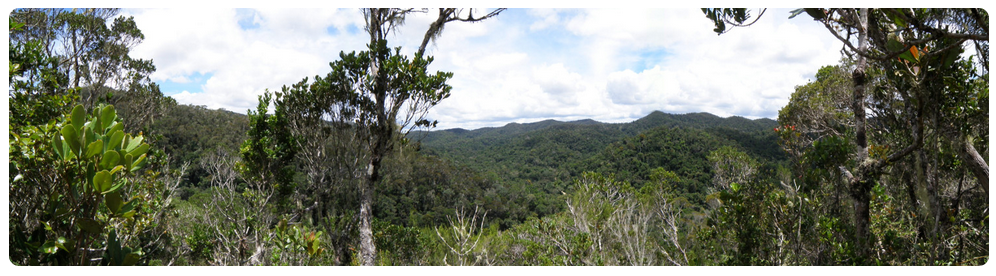
\includegraphics[width=10cm]{figs/Banniere} \small{Ghislain
VIEILLEDENT$^{1}$\hspace{0.25cm}Thomas ARSOUZE$^{1}$\hspace{0.25cm}FAO
team$^{2}$} \vspace{0.25cm} {\scriptsize \begin{tabular}{l} $[1]$
\textbf{Cirad} UMR AMAP, $[2]$ \textbf{FAO} Rome et l'Amérique latine
\end{tabular} } 
\includegraphics[width=0.8\textwidth]{figs/partners_logos}
\end{center} \end{frame} }


\placelogotrue
\begin{frame}
  \N- Titre du cadre{Outline}
  \begin{columns}[c]
    \begin{column}{0.5\largeur du texte} \tableofcontents[sections=1] \vspace{0.5cm}
\tableofcontents[sections=2] \vspace{0.5cm} \tableofcontents[sections=3]
    \end{column}
    \begin{column}{0.5\largeur du texte} \tableofcontents[sections=4] \vspace{0.5cm}
\tableofcontents[sections=5]
    \end{column}
  \end{columns}
\end{frame}
\placelogofalse

\section{Le plugin QGIS deforisk}
\label{sec:org33875a8}

\subsection{Objectif et spécificités}
\label{sec:org2b48526}

\begin{frame}[label={sec:org9b9dfa0}]{Aims}
\begin{itemize}
\item Fournir \textbf{un outil} pour créer et comparer \textbf{les cartes des
risques de déforestation}.
\item Au niveau \textbf{jurisdictional}.
\item Suivre \textbf{la méthodologie de Verra} pour la certification.
\item \textbf{Attribution de la déforestation} à des projets relevant de la
juridiction.
\end{itemize}
\end{frame}

\begin{frame}[label={sec:org670f662}]{Specificities}
\begin{itemize}
\item Open-source et basé sur Python : transparence, reproductibilité.
\item Efficace sur le plan informatique :
\begin{itemize}
\item Traitement de la trame par blocs.
\item Exécution de tâches en parallèle.
\end{itemize}
\item Indépendant du système d'exploitation : Windows, Linux, MacOS.
\item Il devrait fonctionner sur n'importe quel ordinateur aux performances
moyennes.
\item Modèles statistiques alternatifs performants (iCAR).
\item Entièrement documenté et traduit (anglais, espagnol, français).
\item Aide à la préparation des données.
\item Il devrait être (relativement) facile à utiliser.
\end{itemize}
\end{frame}

\begin{frame}[label={sec:orgad092f5},fragile]{Python based}
 The \texttt{deforisk} plugin relies on four Python packages developed
specifically for modelling deforestation:

\begin{itemize}
\item \texttt{geefcc}: créer des cartes de changement de couverture forestière à
partir de Google Earth Engine (GEE).
\item \texttt{pywdpa}: téléchargement des zones protégées à partir de la base de
données mondiale sur les zones protégées (WDPA).
\item \texttt{forestatrisk}: modéliser la déforestation et prédire la
déforestation spatiale.
\item \texttt{riskmapjnr}: cartes de risques suivant les méthodologies Verra JNR.
\end{itemize}

\begin{center}
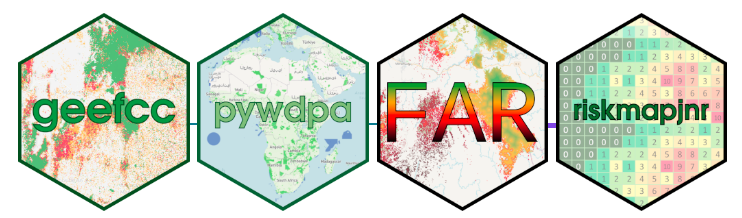
\includegraphics[width=0.7\textwidth]{figs/logos-packages.png}
\end{center}
\end{frame}

\begin{frame}[label={sec:org3f9636c},fragile]{Processing raster by blocks}
 \begin{itemize}
\item Les fichiers matriciels des changements du couvert forestier et des
variables explicatives peuvent occuper un espace de plusieurs gigaoctets sur
le disque.
\item Le traitement en mémoire de trames aussi importantes peut s'avérer
prohibitif sur les ordinateurs disposant d'une mémoire vive limitée.
\item Les fonctions utilisées dans le plugin \texttt{deforisk} traitent les grands
rasters par blocs de pixels représentant des sous-ensembles de données
raster.
\item Cela rend le calcul efficace et permet une faible utilisation de la mémoire.
\end{itemize}

\begin{center}
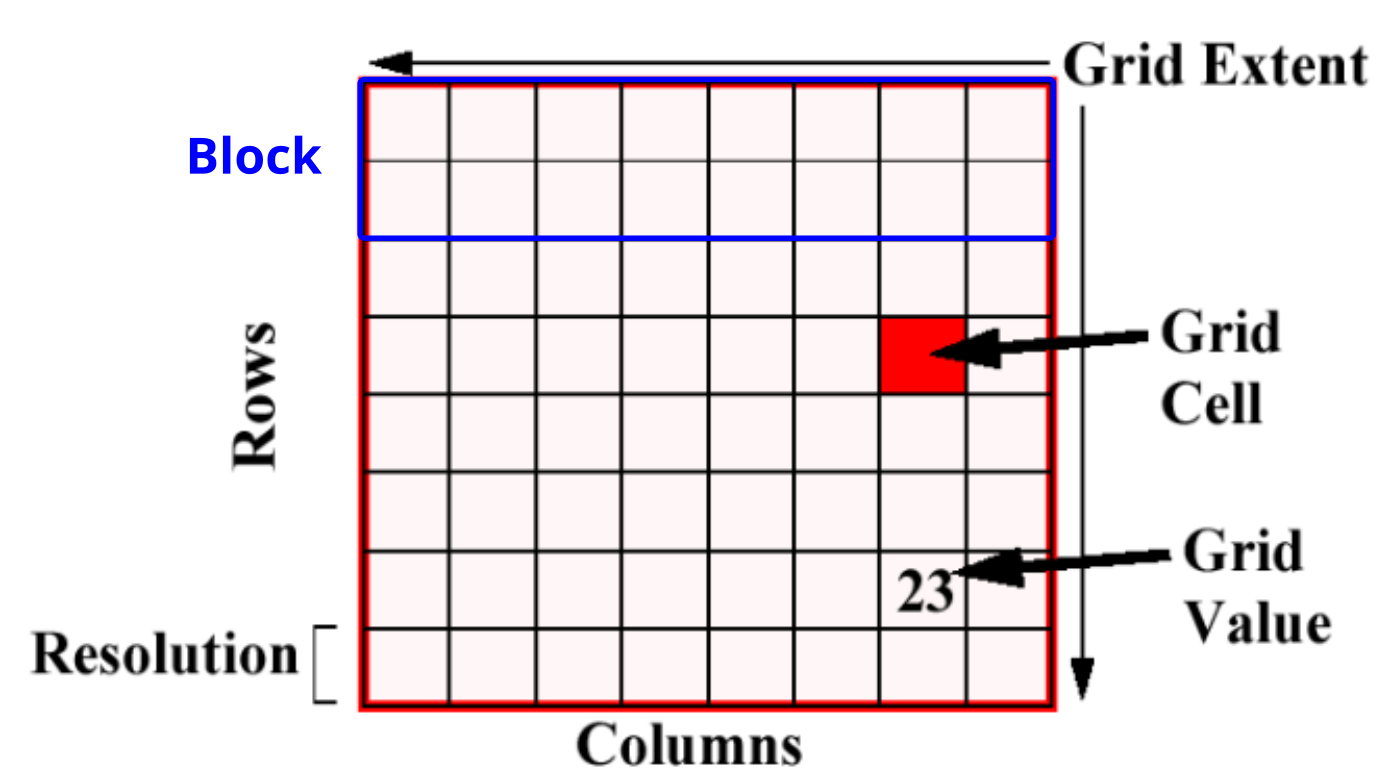
\includegraphics[width=6cm]{figs/raster_block.png}
\end{center}
\end{frame}

\begin{frame}[label={sec:org87726f7},fragile]{Running tasks in parallel}
 \begin{itemize}
\item L'approche de pointe pour sélectionner la meilleure carte des risques
implique des tâches répétitives (modèle, périodes).
\item Pour économiser du temps de calcul, le plugin{deforisk} utilise le
gestionnaire de tâches de QGIS.
\item Permet d'effectuer plusieurs analyses en parallèle.
\end{itemize}

\vspace{0.25cm}

\begin{center}
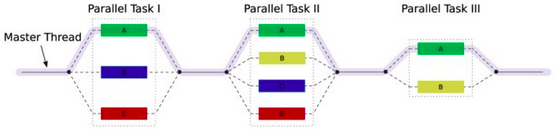
\includegraphics[width=9cm]{figs/parallel_tasks.png}
\end{center}
\end{frame}

\subsection{Site web et documentation}
\label{sec:orgd6a1b3f}

\begin{frame}[label={sec:orgb622ffa}]{Site web et documentation}
The website includes all the documentation to use the plugin:

\begin{itemize}
\item \href{https://deforisk-qgis-plugin.org/installation.html}{Installation
page}: How to install the plugin?
\item \href{https://deforisk-qgis-plugin.org/plugin\_api.html}{Plugin API page}:
What is the meaning of each parameter?
\item \href{https://deforisk-qgis-plugin.org/get\_started.html}{Get started
page}. How to start using the plugin on a small area of interest?
\item \href{https://deforisk-qgis-plugin.org/articles.html}{Articles' page}. How
can I use the plugin for specific cases (subnational jurisdictions, user's
data)?
\item \href{https://deforisk-qgis-plugin.org/articles/references.html}{Page de
références} : Une page contenant des documents de référence, y compris des
présentations.
\end{itemize}

\begin{columns}
\begin{column}{0.5\columnwidth} \flushright \url{https://deforisk-qgis-plugin.org}
\end{column}
\begin{column}{0.5\columnwidth}
\begin{center}
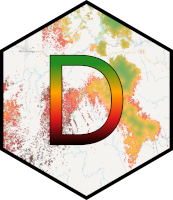
\includegraphics[width=2cm]{figs/logo-deforisk.png}
\end{center}
\end{column}
\end{columns}
\end{frame}

\subsection{Installation}
\label{sec:org724424f}

\begin{frame}[label={sec:org540feec},fragile]{Installation}
 Reduced number of steps for installing the plugin:

\begin{itemize}
\item Installez QGIS et GDAL sur votre système (en utilisant \texttt{OSGeo4W} sur
Windows).
\item Installez les paquets Python \texttt{forestatrisk} et \texttt{riskmapjnr} à
l'aide de pip.
\item \href{https://github.com/ghislainv/deforisk-qgis-plugin/archive/refs/heads/main.zip}{Télécharger}
et installer le plugin \texttt{deforisk} de QGIS.
\item (Systèmes de type Unix uniquement : installer les outils OSM).
\end{itemize}

\begin{center}
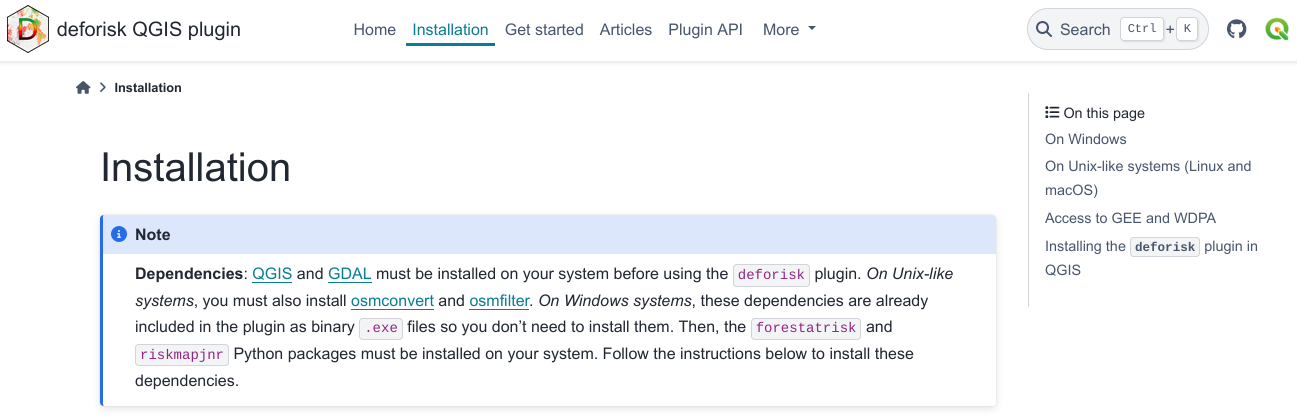
\includegraphics[width=0.9\textwidth]{figs/installation.png}
\end{center}
\end{frame}

\section{Préparation des données}
\label{sec:org43b0b1c}

\subsection{Obtenir des variables}
\label{sec:org4540d1c}

\begin{frame}[label={sec:orgf7a27fd}]{Obtenir des variables}
\begin{columns}
\begin{column}{0.5\columnwidth}
\begin{itemize}
\item Fonctions permettant de préparer les données pour la modélisation de la
déforestation.
\item Deux sources différentes pour \textbf{le changement de couvert forestier}
(GFC ou TMF).
\item Variables explicatives spatiales décrivant \textbf{l'accessibilité à la
forêt} et \textbf{l'occupation des sols} (altitude, pente, distance par
rapport aux routes, aux zones protégées, etc.)
\end{itemize}
\end{column}

\begin{column}{0.5\columnwidth}
\begin{center}
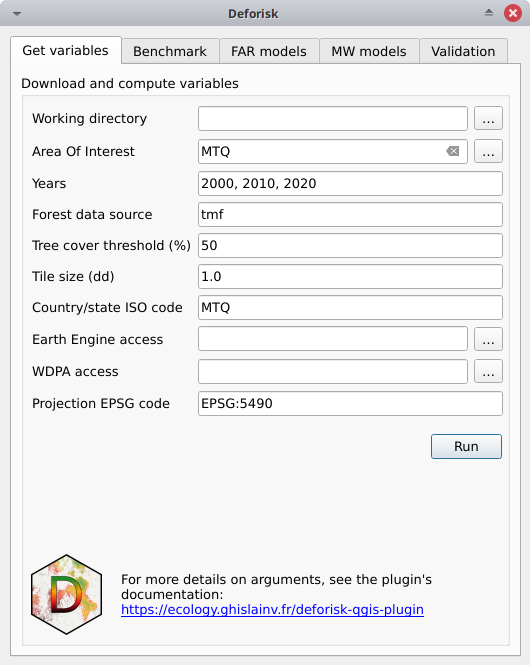
\includegraphics[width=5cm]{figs/plugin_api/interface_variables.png}
\end{center}
\end{column}
\end{columns}
\end{frame}

\subsection{Données sur l'évolution du couvert forestier}
\label{sec:org7f33108}

\begin{frame}[label={sec:orgaeedc82}]{GFC dataset}
\begin{itemize}
\item Hansen et al.  2013.
\item Ensemble de données globales englobant tous les types de forêts.
\item Couvert arboré et perte annuelle de couvert arboré.
\item Résolution de 30 m, à partir de 2000.
\item Données : \url{https://glad.earthengine.app/view/global-forest-change}
\end{itemize}

\begin{center}
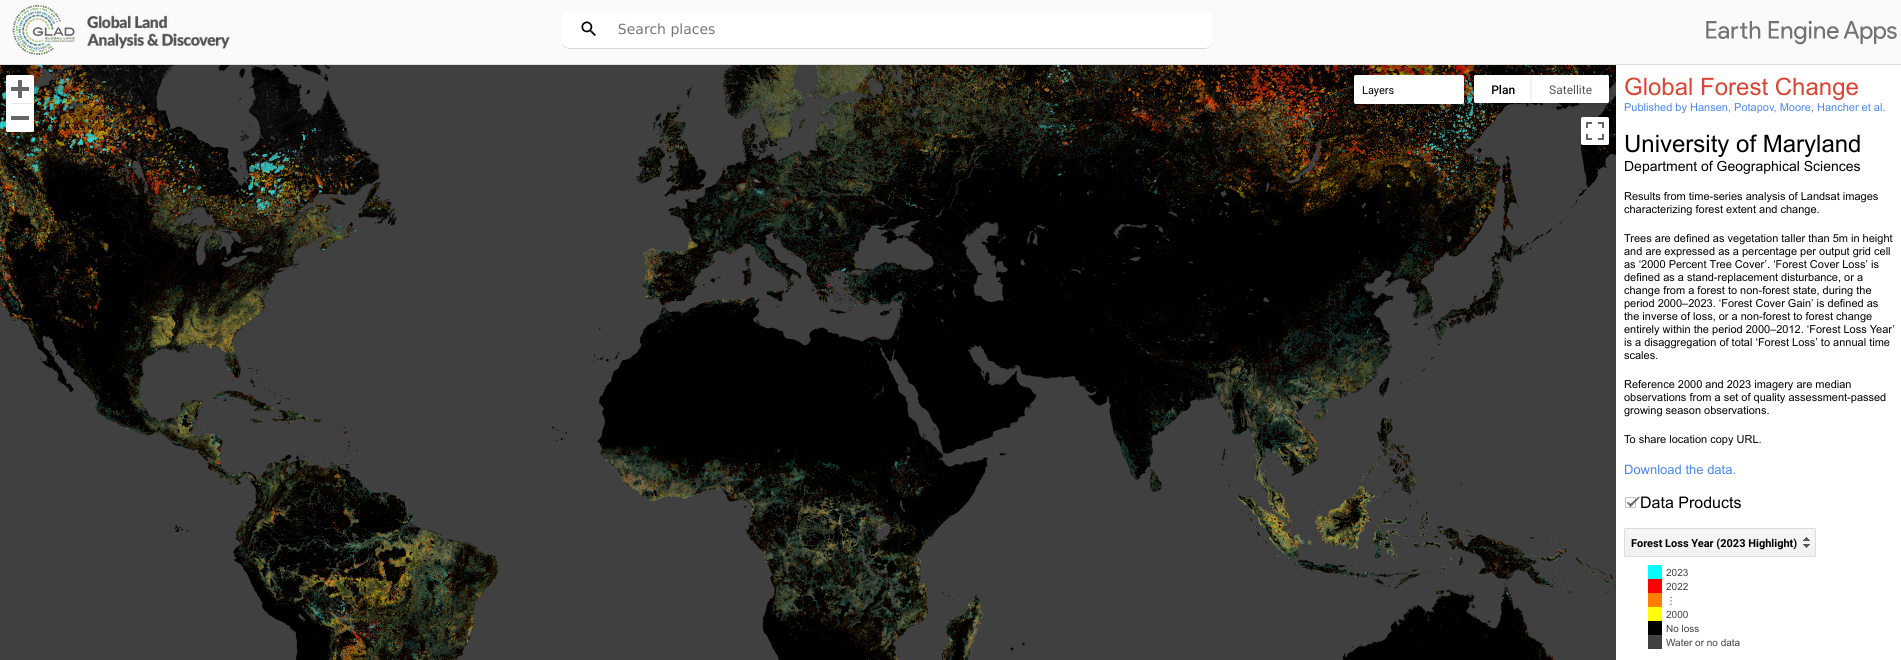
\includegraphics[width=\textwidth]{figs/gfc.png}
\end{center}
\end{frame}

\begin{frame}[label={sec:org4f33ca0}]{TMF dataset}
\begin{itemize}
\item Vancutsem et al.  2021.  Forêts tropicales humides (forêts à feuilles
persistantes, pas de forêts sèches à feuilles caduques).
\item Résolution de 30 m, à partir de 1990.
\item La déforestation tropicale a été sous-estimée (-33% en 2000--2012, Hansen et
al.  2013), en particulier en Afrique.
\item Données : \url{https://forobs.jrc.ec.europa.eu/TMF/}.
\end{itemize}

\vspace{0.25cm}

\begin{center}
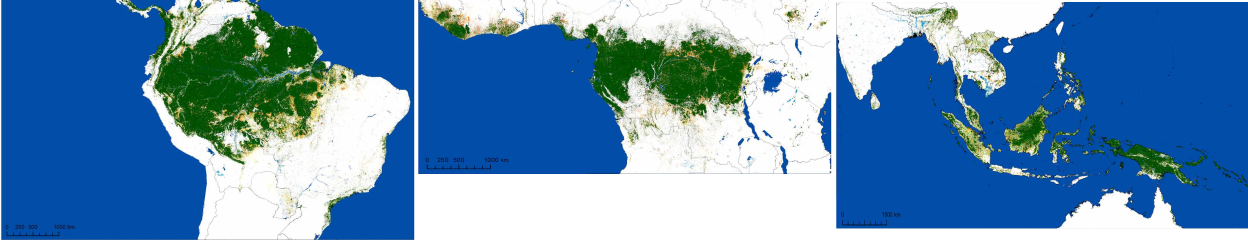
\includegraphics[width=\textwidth]{figs/Vancutsem2021-maps-wide.png}
\end{center}
\end{frame}

\begin{frame}[label={sec:orgd0bbec4}]{TMF dataset}
\begin{itemize}
\item Suffisamment précis pour identifier visuellement les causes de la
déforestation (exploitation forestière, incendies, agriculture)
\end{itemize}

\begin{center}
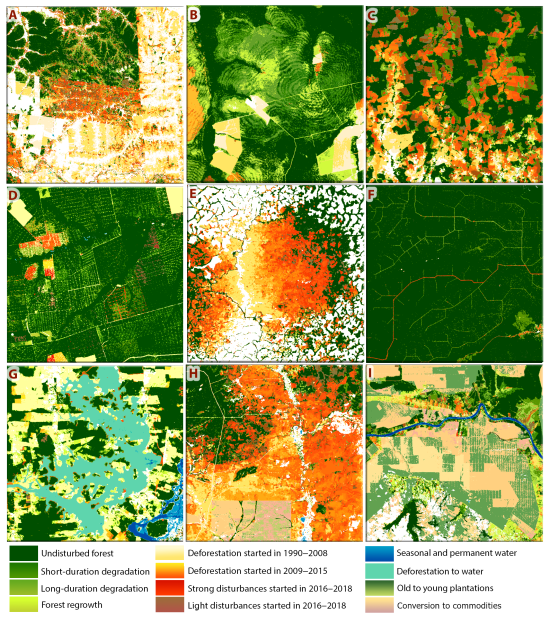
\includegraphics[width=0.5\textwidth]{figs/Vancutsem2021-patterns.png}
\end{center}
\end{frame}

\subsection{Variables explicatives spatiales}
\label{sec:org3a75228}

\begin{frame}[label={sec:org8b6e56b}]{Spatial variables}
The plugin helps computing eight explanatory variables.

\begin{center}
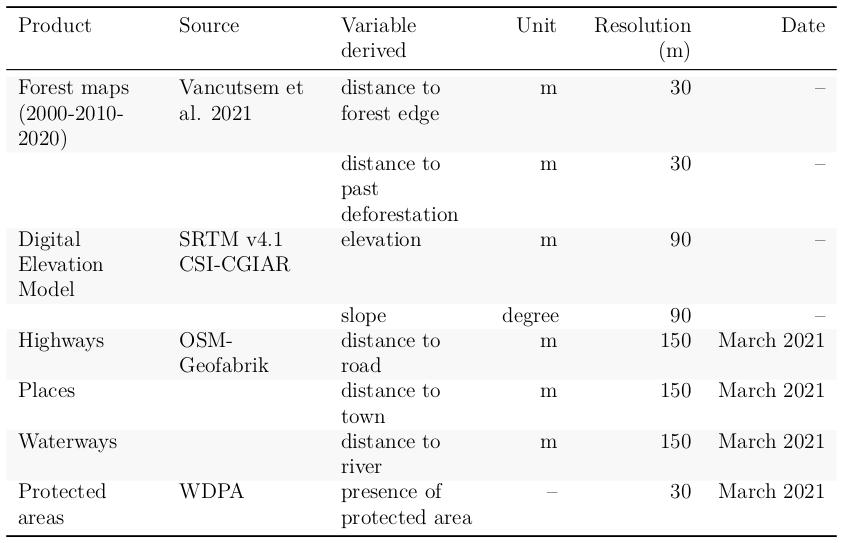
\includegraphics[width=0.75\textwidth]{figs/variables-tab.png}
\end{center}
\end{frame}

\begin{frame}[label={sec:orgbd91830}]{Spatial variables}
\begin{center}
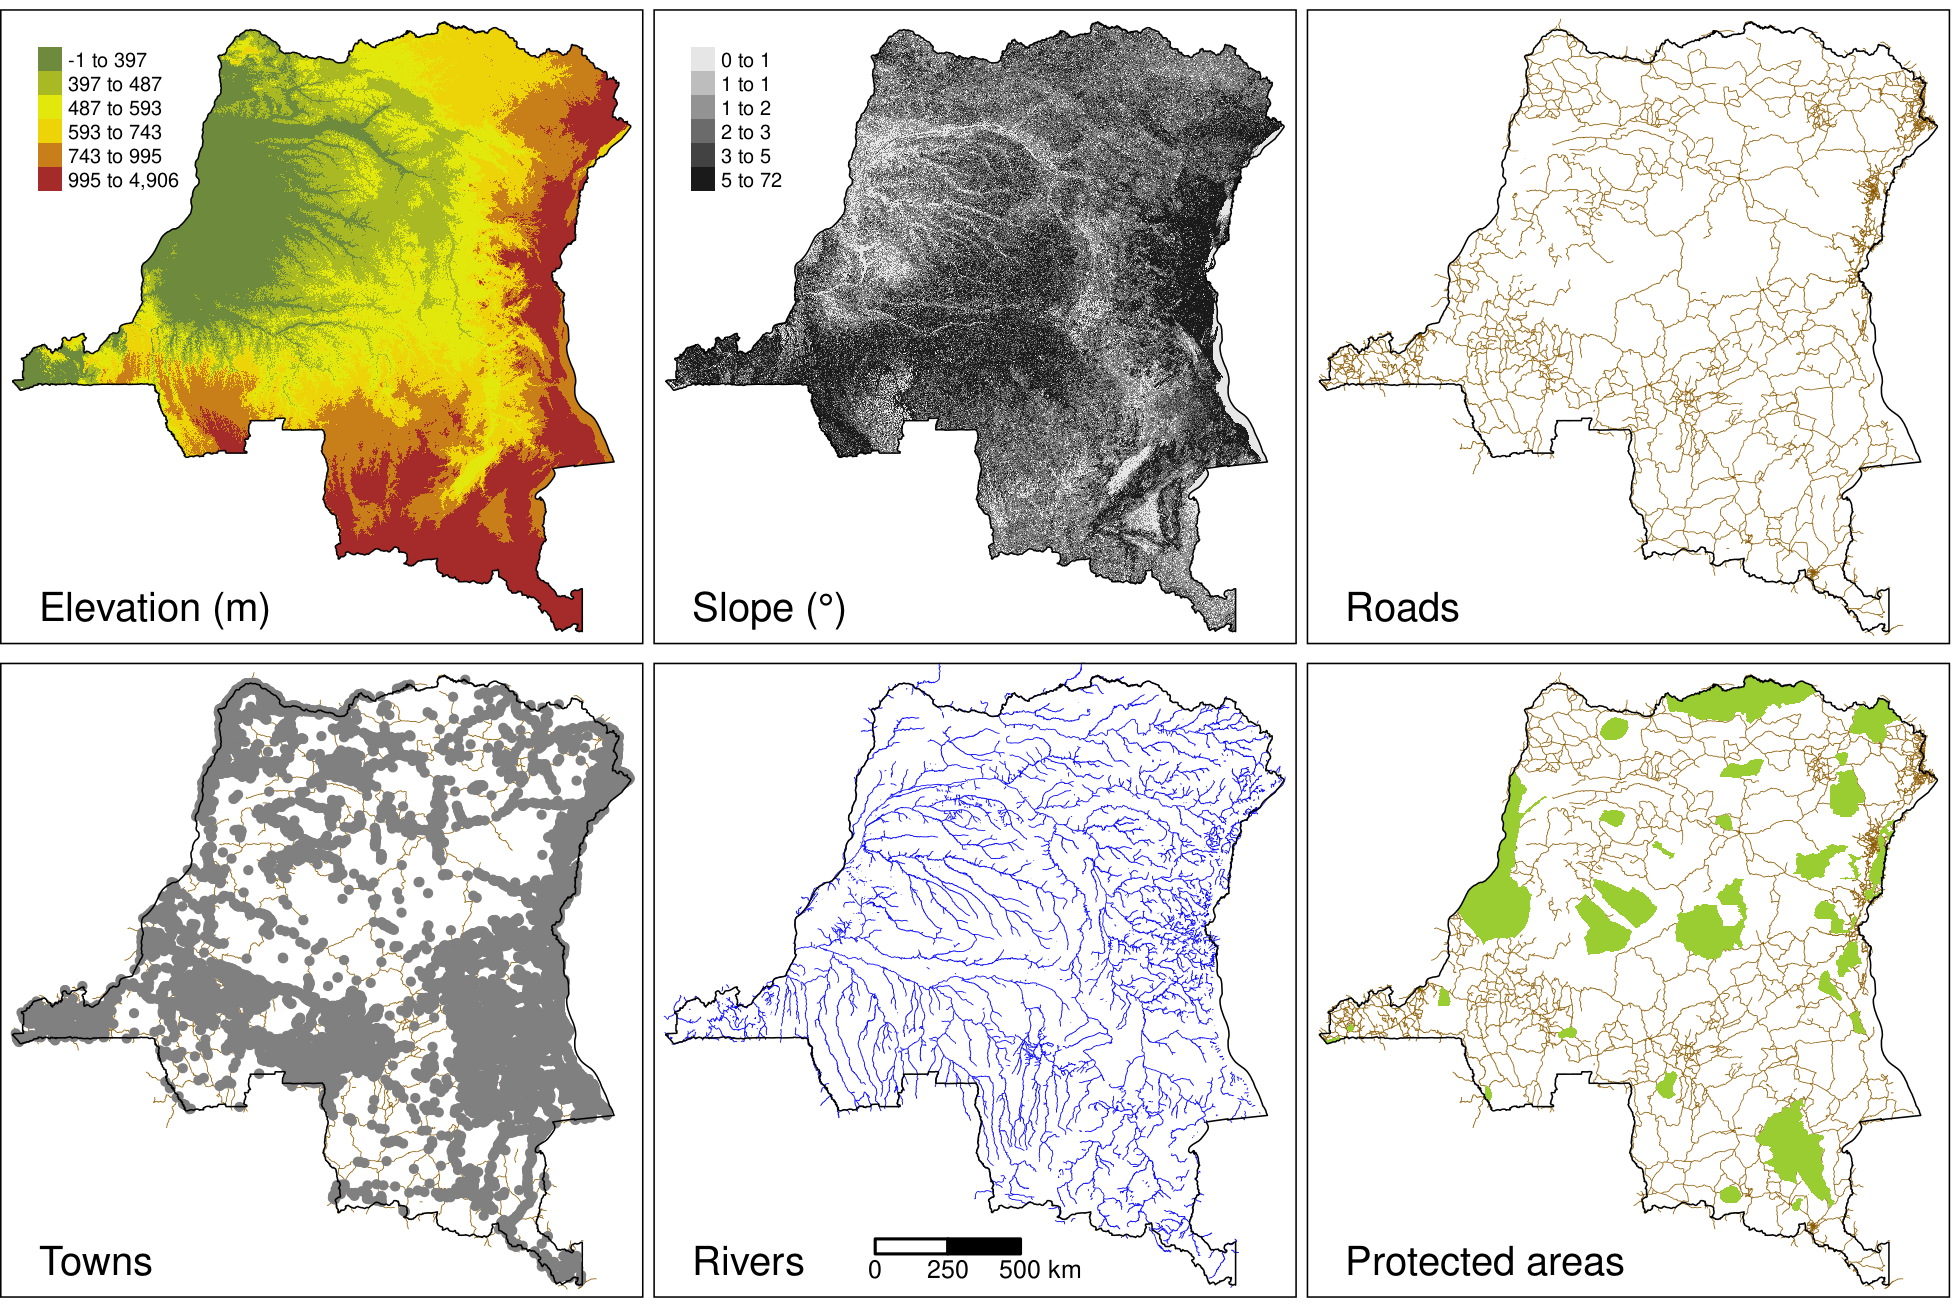
\includegraphics[width=0.8\textwidth]{figs/sm/var.png}
\end{center}

\centering \textbf{Variables explicatives spatiales en RDC}
\end{frame}

\begin{frame}[label={sec:orgd6e5a80}]{Roads}
\begin{itemize}
\item OpenStreetMap (OSM)
\item les autoroutes, les routes principales, les routes secondaires et les routes
tertiaires.
\item 3,6 millions de routes grâce à OSM
\end{itemize}

\begin{center}
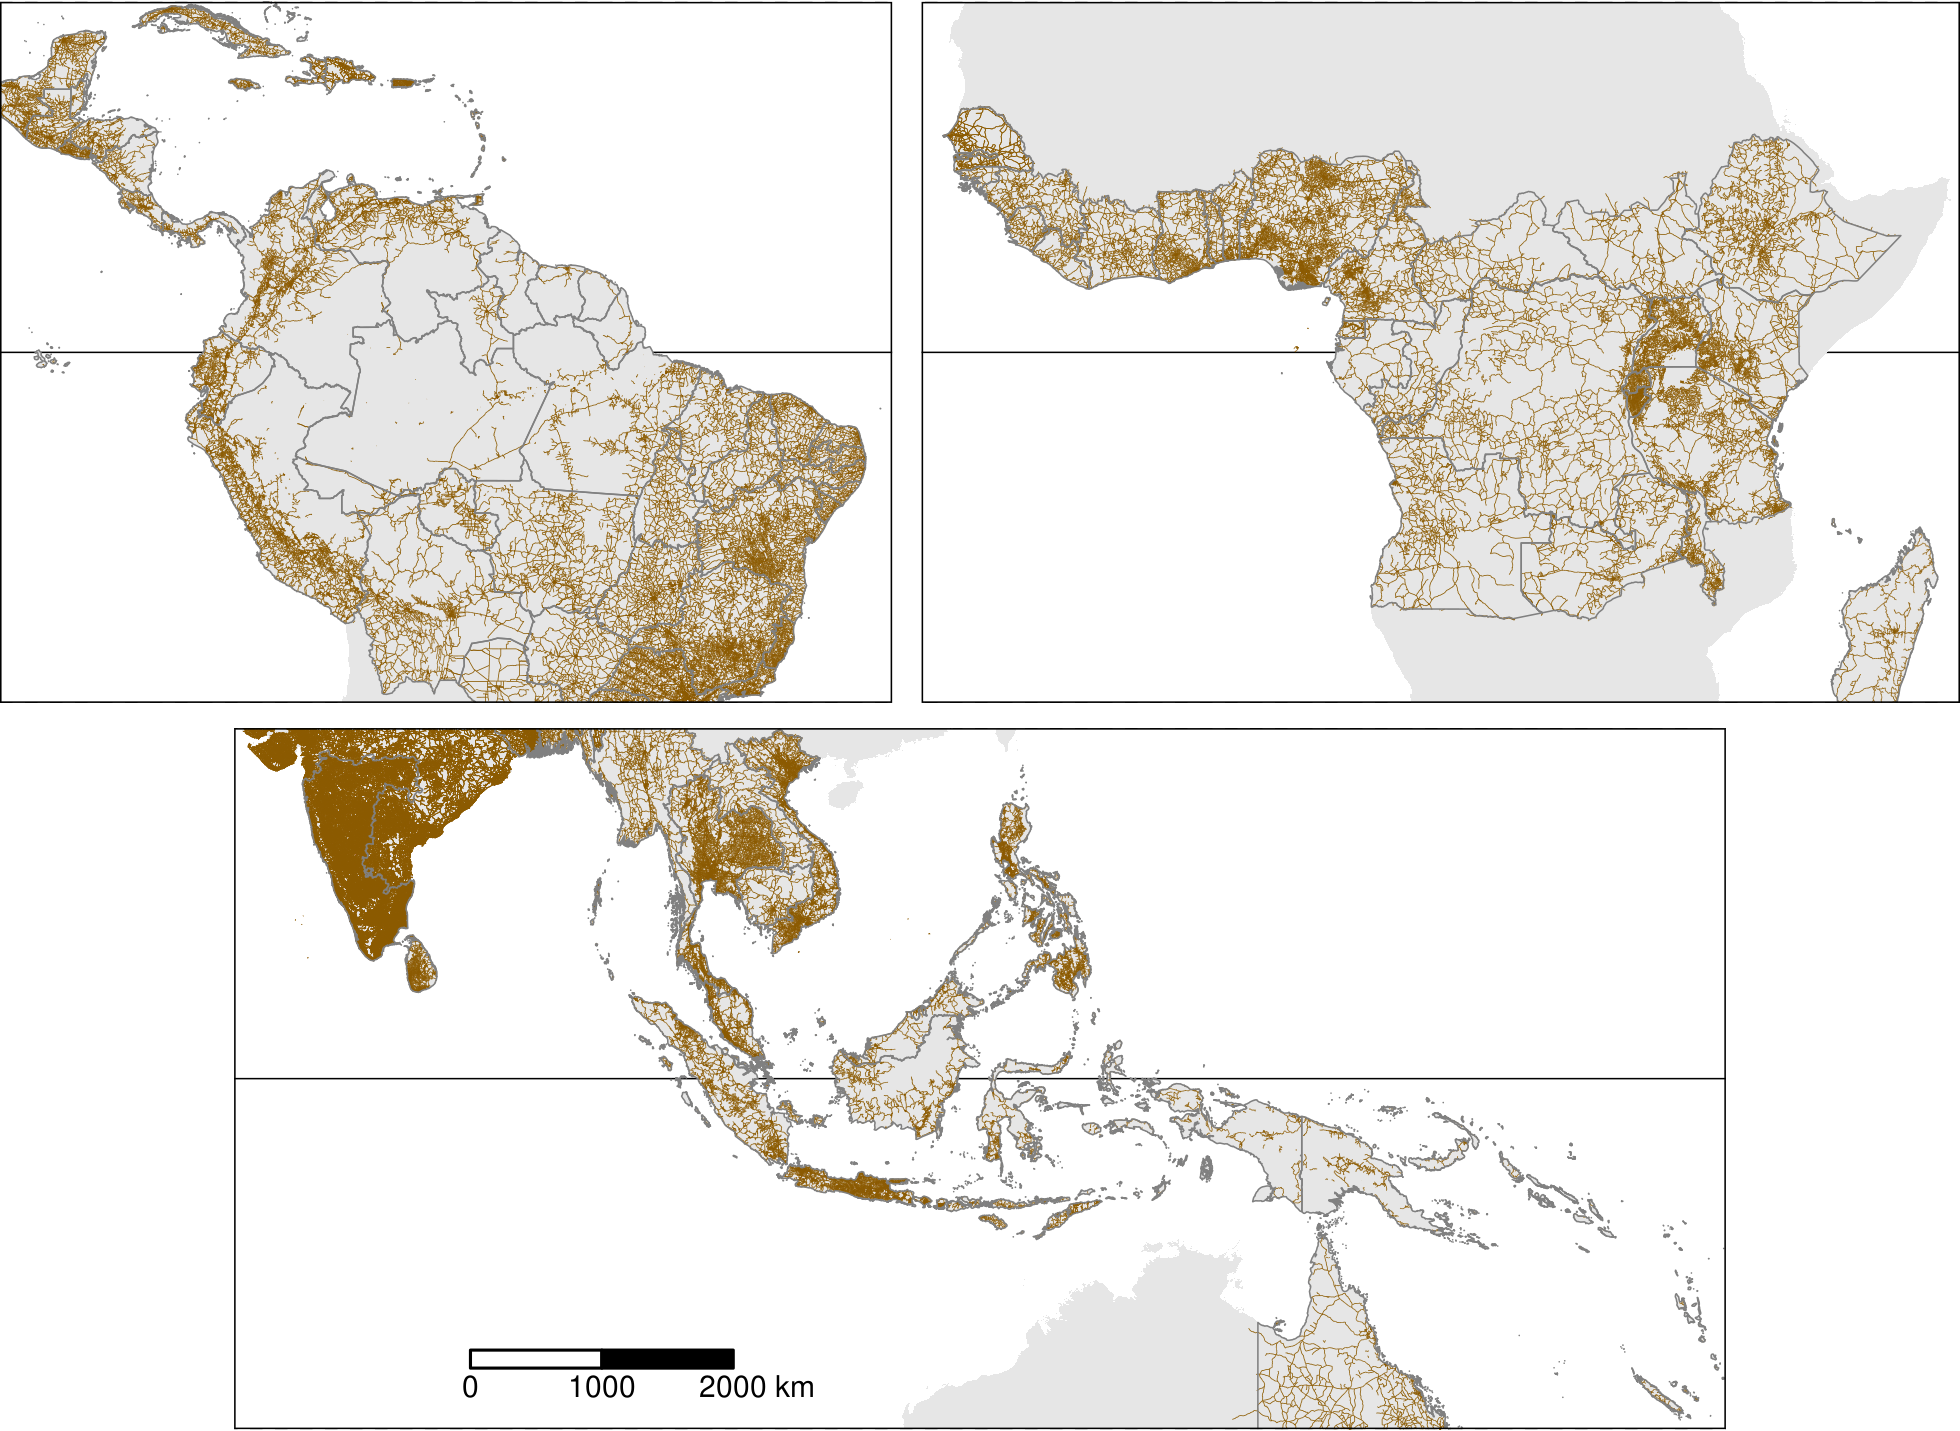
\includegraphics[width=0.7\textwidth]{figs/sm/roads.png}
\end{center}
\end{frame}

\begin{frame}[label={sec:org0304202}]{Protected areas}
\begin{itemize}
\item Statut de l'AP : "Désigné", "Inscrit", "Établi" ou "Proposé".
\item 85 000 zones protégées de la WDPA.
\end{itemize}

\begin{center}
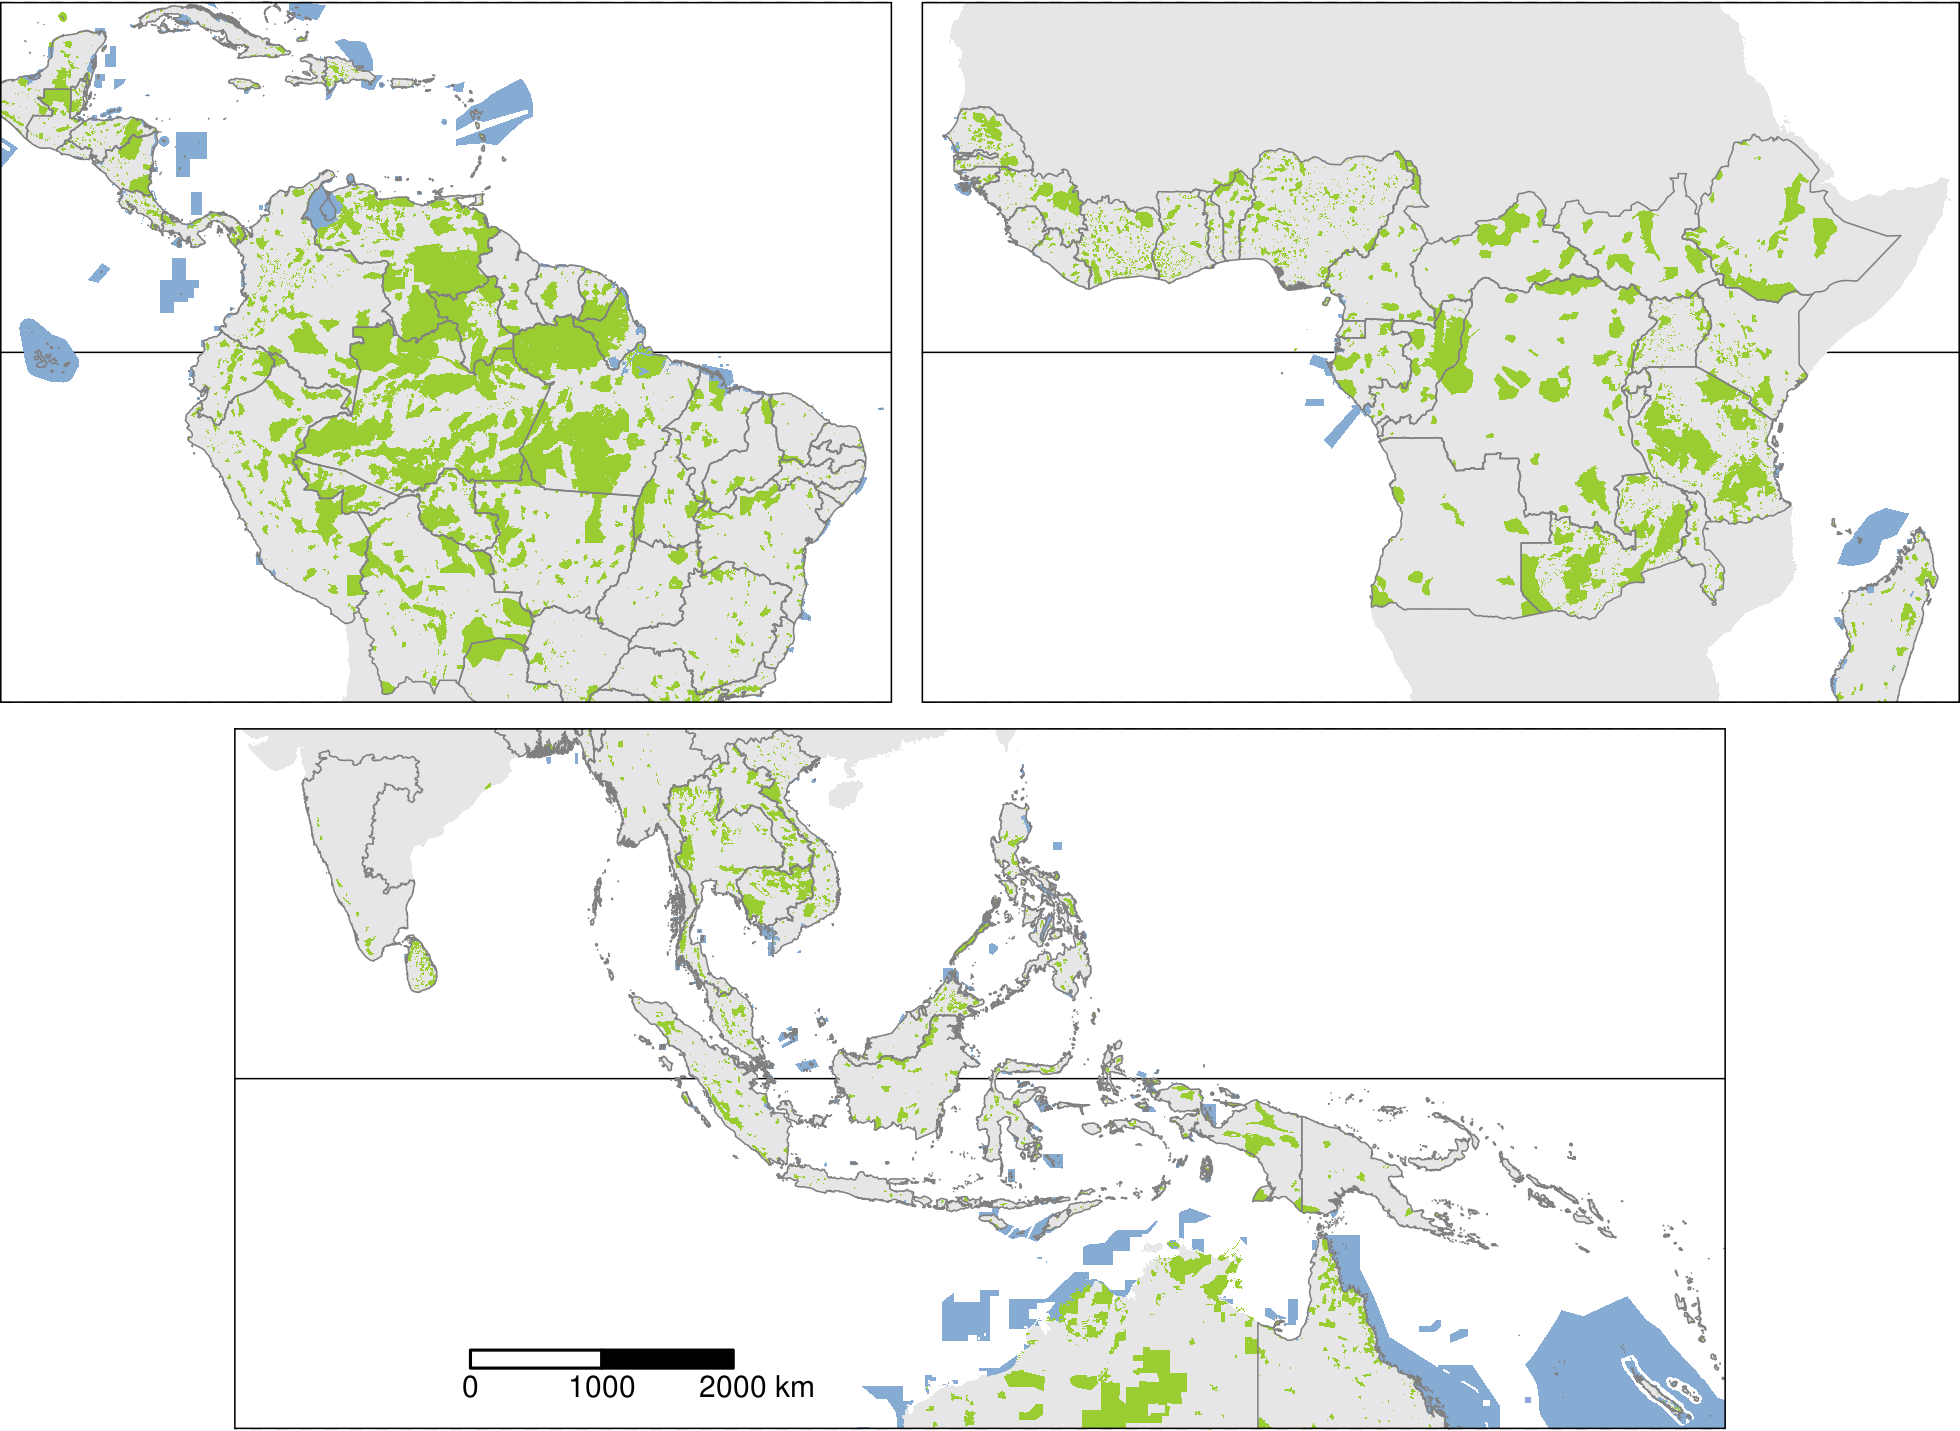
\includegraphics[width=0.7\textwidth]{figs/sm/pa.png}
\end{center}
\end{frame}

\section{Modèles et validation}
\label{sec:orge1c0621}

\subsection{Modèle de référence}
\label{sec:org4d6d90a}

\begin{frame}[label={sec:org46860d4}]{Modèle de référence}
\begin{columns}
\begin{column}{0.5\columnwidth}
\begin{itemize}
\item Modèle de référence ou modèle de référence.
\item Un modèle de déforestation raisonnablement bon (mieux qu'un modèle nul).
\item En supposant une \emph{décroissance de la déforestation avec la distance à
la lisière de la forêt} (communément admise).
\item Et un \emph{modèle différent selon les juridictions} (variabilité
régionale).
\item Voir présentation \textbf{Cirad et
FAO}.
2024.
\href{https://deforisk-qgis-plugin.org/\_static/references/Cirad2024-riskmap-verra.pdf}{Cartes
de risques juridictionnels pour l'allocation de la déforestation}.
\end{itemize}
\end{column}

\begin{column}{0.5\columnwidth}
\begin{center}
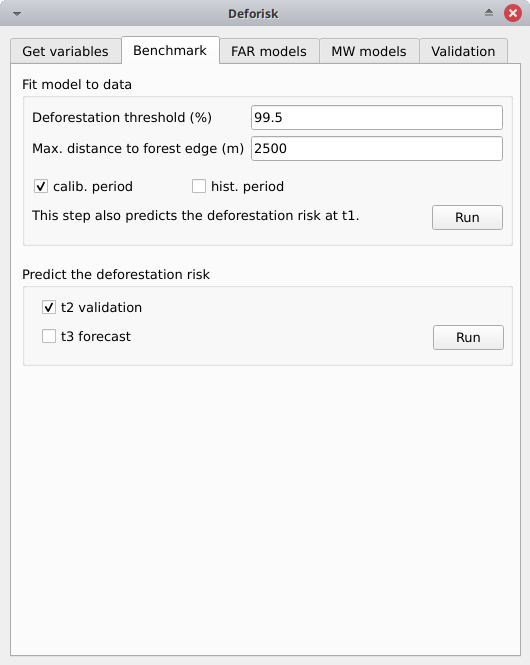
\includegraphics[width=5cm]{figs/plugin_api/interface_benchmark.png}
\end{center}  
\end{column}
\end{columns}
\end{frame}

\subsection{Modèles de risque forestier}
\label{sec:org0b990cb}

\begin{frame}[label={sec:org989b75f}]{Modèles de risque forestier}
\begin{columns}
\begin{column}{0.5\columnwidth}
\begin{itemize}
\item Trois modèles statistiques : iCAR, GLM, RF.
\item iCAR : Régression logistique avec effets aléatoires spatiaux (processus
iCAR).
\item GLM : Generalized Linear Model, régression logistique simple (sans effets
aléatoires).
\item Modèle Random Forest : arbres de régression aléatoires.
\item Modèles statistiques basés sur un échantillon d'observations.
\end{itemize}
\end{column}

\begin{column}{0.5\columnwidth}
\begin{center}
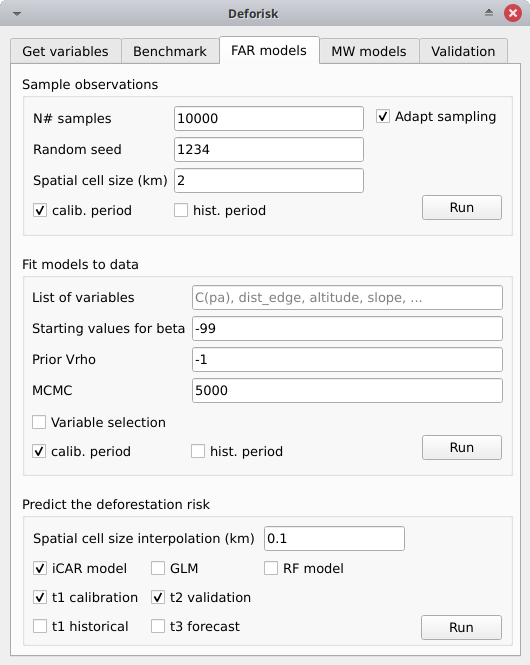
\includegraphics[width=5cm]{figs/plugin_api/interface_far_models.png}
\end{center}  
\end{column}
\end{columns}
\end{frame}

\begin{frame}[label={sec:org0bbacb1}]{Sampling for FAR models}
\begin{itemize}
\item Nous considérons l'évolution du couvert forestier entre \(t\N) et \N(t+1\N).
\item Échantillonnage stratifié entre les pixels déboisés et non déboisés.
\item Nombre total de points proportionnel au couvert forestier (de 20 000 à 100
000 points par zone d'étude).
\end{itemize}

\begin{center}
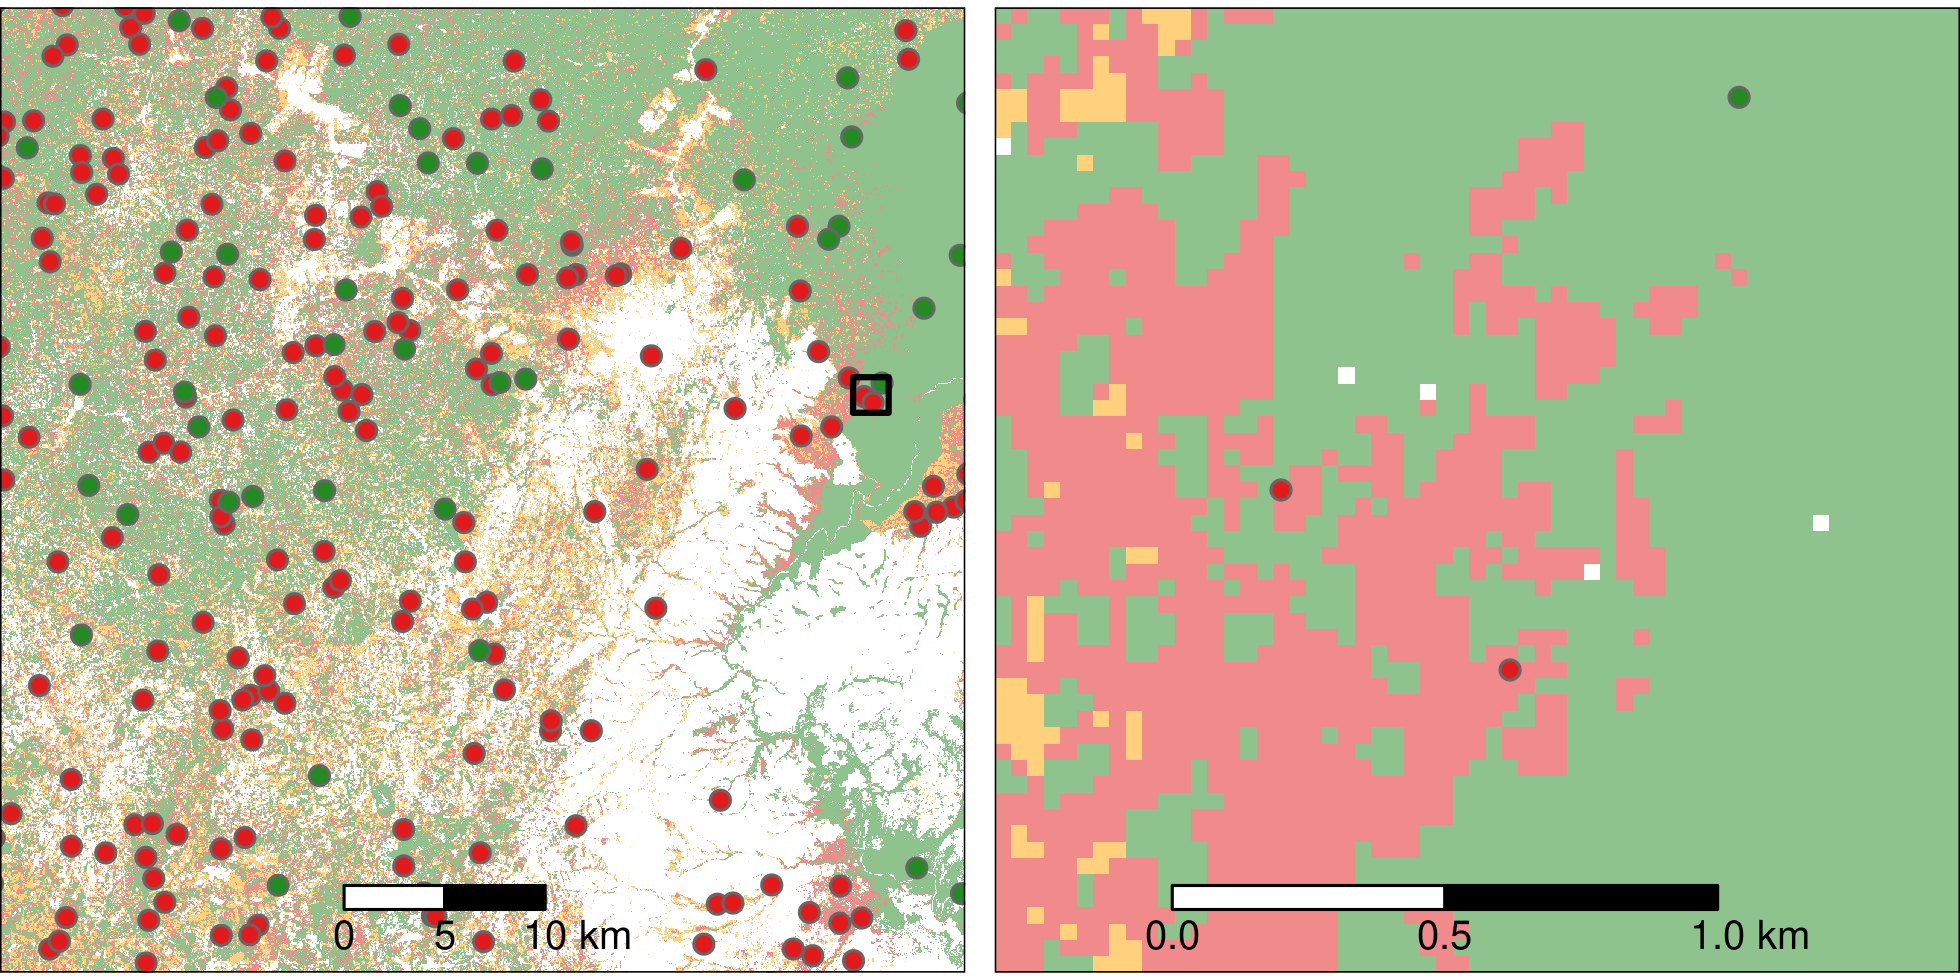
\includegraphics[width=0.7\textwidth]{figs/sm/sample.png}
\end{center}
\end{frame}

\begin{frame}[label={sec:orgd30ce3c}]{iCAR model}
\begin{columns}
\begin{column}{0.5\columnwidth} Modèle de régression logistique avec processus iCAR :

\begin{equation*}
\begin{split}
  y_i \sim \mathcal{B}ernoulli(\theta_i)\text{logit}(\theta_i) = \alpha + X_i
\beta + \rho_{j(i)}\\rho_{j(i)} \sim \mathcal{N}ormal(\sum_{j^{\prime}}
\rho_{j^{\prime} / n_j,V_{\rho} / n_j)
\end{split}
\end{equation*}

\textbf{Les effets aléatoires \(\rho_{j(i)}\) permettent de tenir compte de la
variation spatiale résiduelle non prise en compte par les variables du
modèle \(X_i\).}
\end{column}

\begin{column}{0.5\columnwidth}
\begin{center}
\includegraphics[width=\textwidth]{figs/sm/grid.png}
\end{center}

\centering \textbf{Grille carrée de cellules de 10 km sur la RDC}
\end{column}
\end{columns}
\end{frame}

\begin{frame}[label={sec:orge7256cf}]{Spatial random effects}
\begin{center}
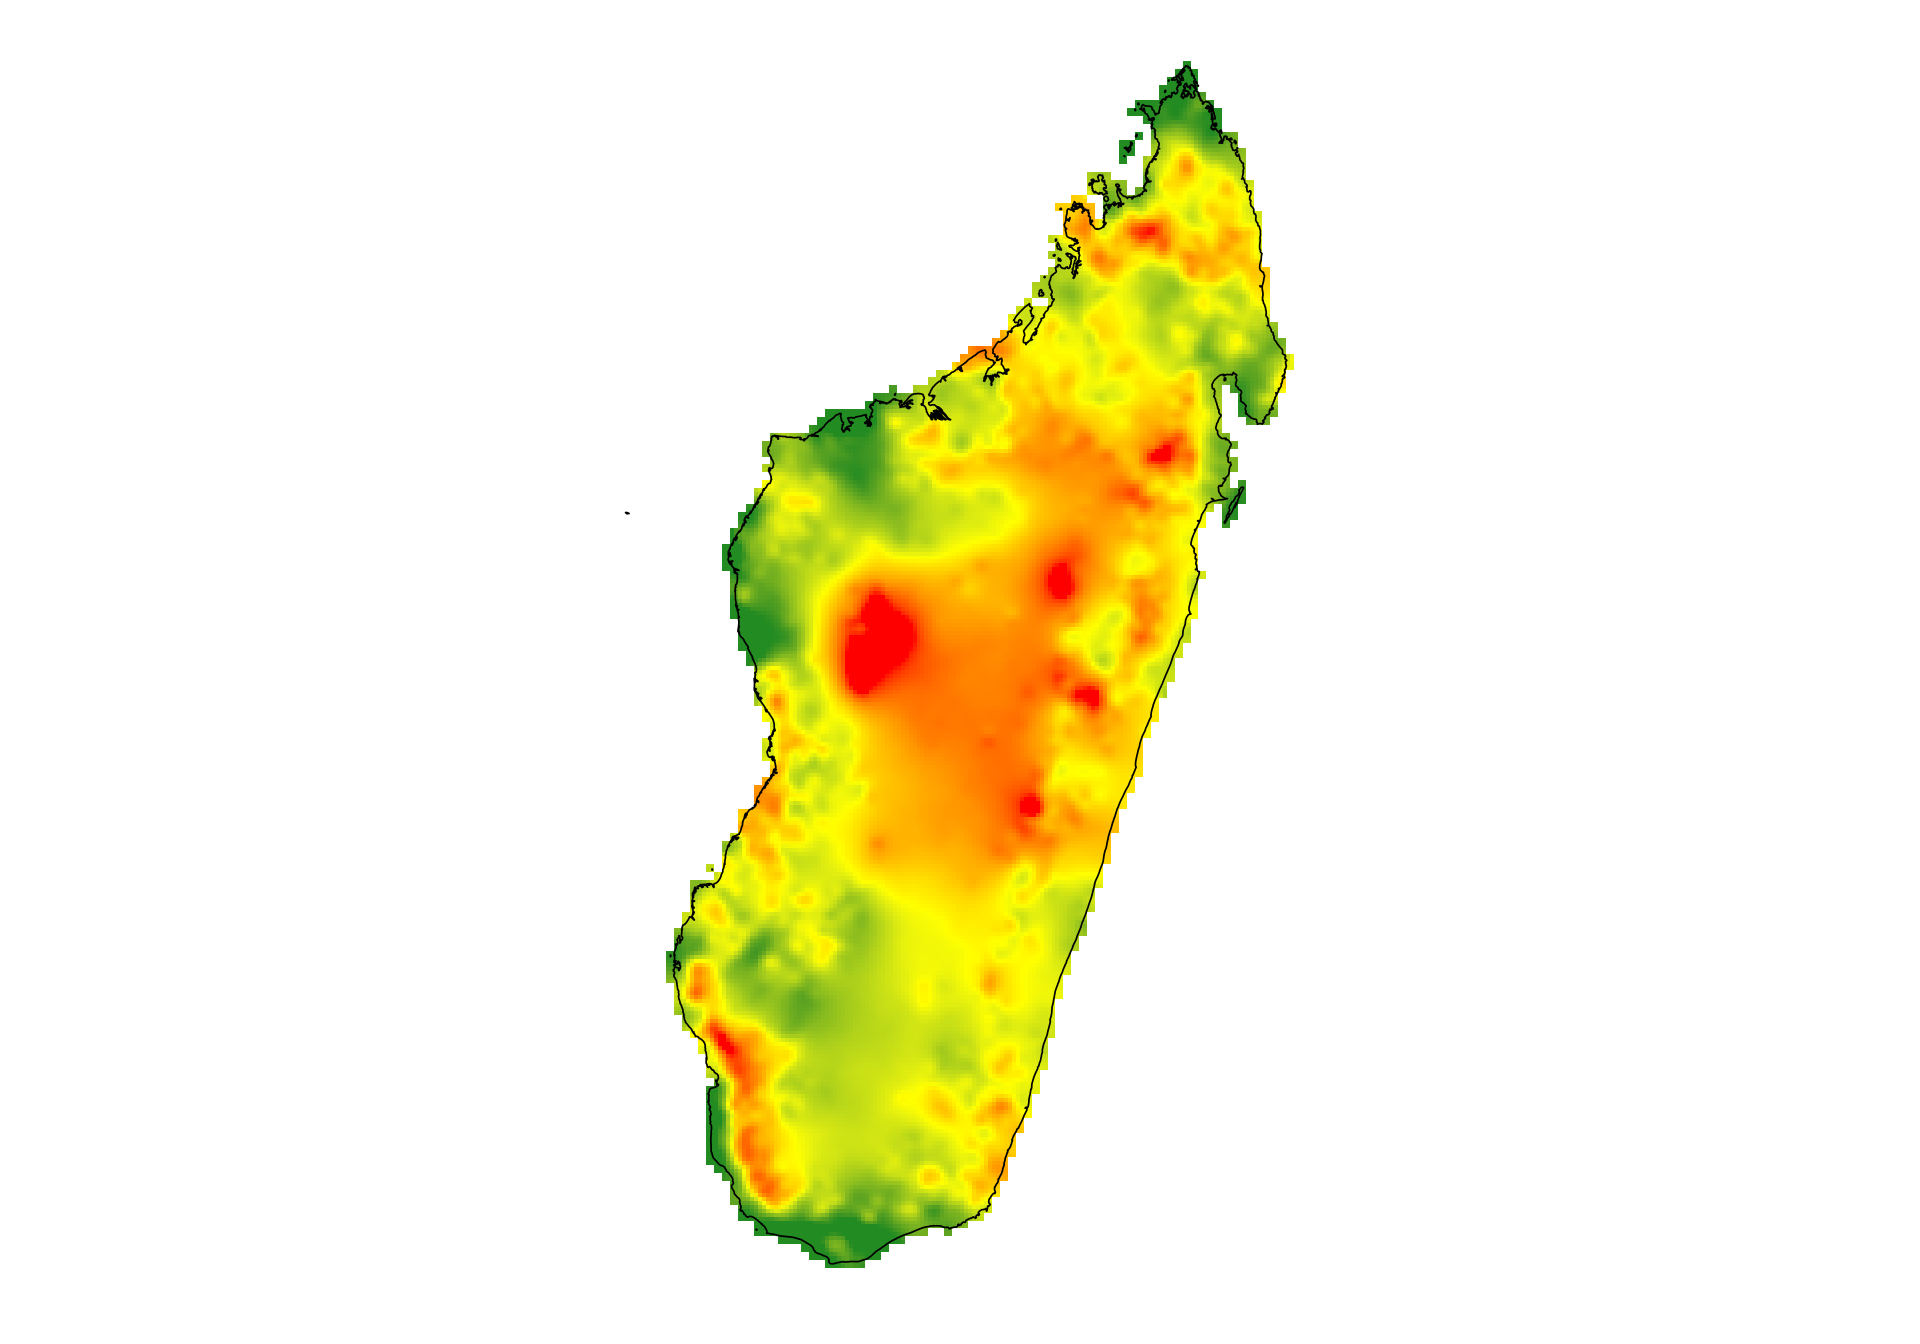
\includegraphics[width=0.6\textwidth]{figs/sm/rho.png}
\end{center}

\centering \textbf{Interpolation des effets spatiaux aléatoires à 1km en RDC}
\end{frame}

\begin{frame}[label={sec:org0f0fda3}]{Spatial probability of deforestation}
\begin{itemize}
\item We use the fitted model to compute the spatial probability of deforestation.
\item Les probabilités dans [0, 1] sont transformées en classes dans [1, 65535].
\end{itemize}

\begin{center}
\includegraphics[width=0.5\textwidth]{figs/sm/prob.png}
\end{center}

\centering \textbf{Probabilité spatiale relative de déforestation en RDC}
\end{frame}

\begin{frame}[label={sec:org599fb42}]{GLM model}
A simple logistic regression model without random effects:

\begin{equation*}
\begin{split}
  y_i \sim \mathcal{B}ernoulli(\theta_i)\\ntext{logit}(\theta_i) = \alpha +
X_i \beta
\end{split}
\end{equation*}

Facile à comparer avec iCAR pour voir l'impact des effets aléatoires
spatiaux.
\end{frame}

\begin{frame}[label={sec:org52dbe2f}]{Random Forest model}
\begin{itemize}
\item Random Forest est un algorithme d'apprentissage automatique d'ensemble.
\item Combine plusieurs arbres de décision pour créer un modèle prédictif plus
robuste et plus précis.
\end{itemize}

\begin{center}
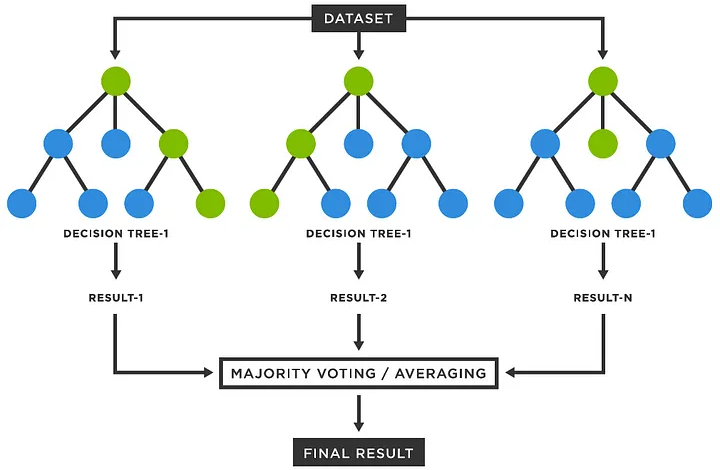
\includegraphics[width=0.7\textwidth]{figs/random_forest.png}
\end{center}
\end{frame}

\begin{frame}[label={sec:orgd707d4f}]{ForestAtRisk in the tropics}
\begin{itemize}
\item \textbf{i.} Considérer la forêt tropicale humide dans \textbf{92} pays (119
zones d'étude)
\item \textbf{ii.} Estimer le taux de déforestation actuel et l'incertitude dans
chaque pays
\item \textbf{iii.} Modéliser le risque spatial de déforestation à partir de
facteurs environnementaux
\item \textbf{iv.} Prévision de la déforestation dans l'hypothèse d'un scénario de
statu quo
\item \textbf{v.} Conséquences en termes d'émissions de carbone
\end{itemize}

\vspace{0.5cm}
\begin{center}
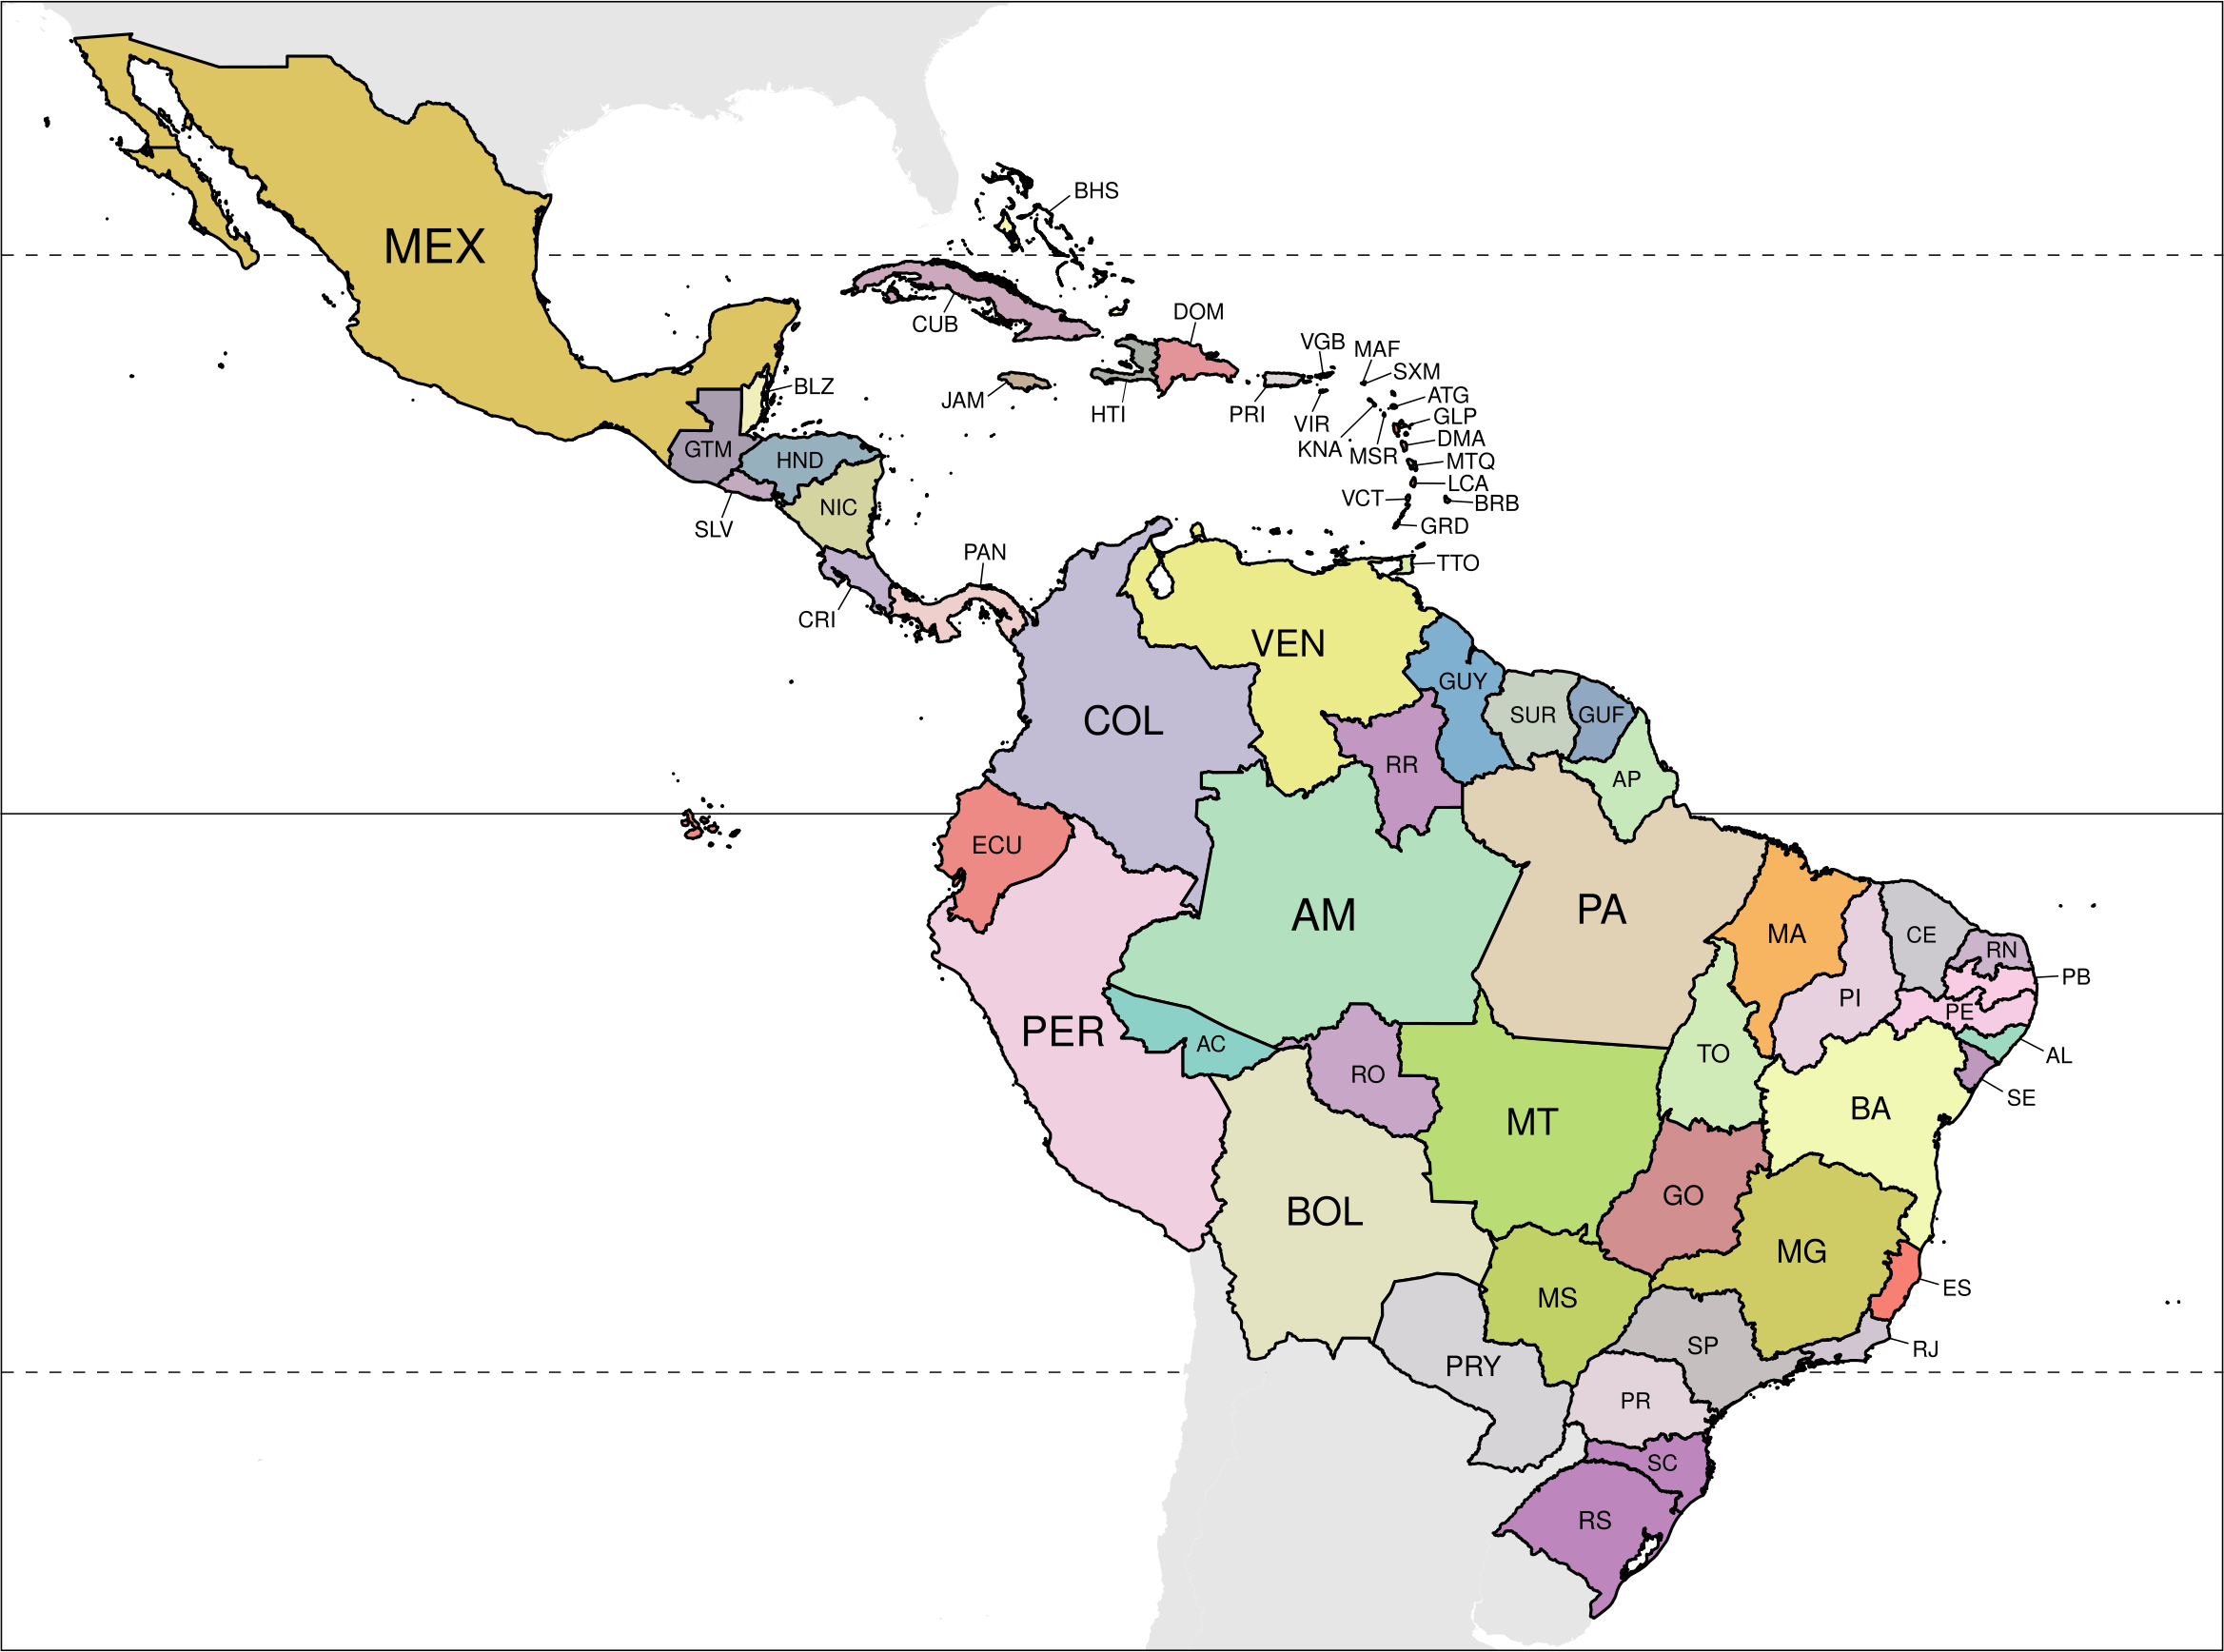
\includegraphics[width=0.32\textwidth]{figs/sm/study_areas_America}
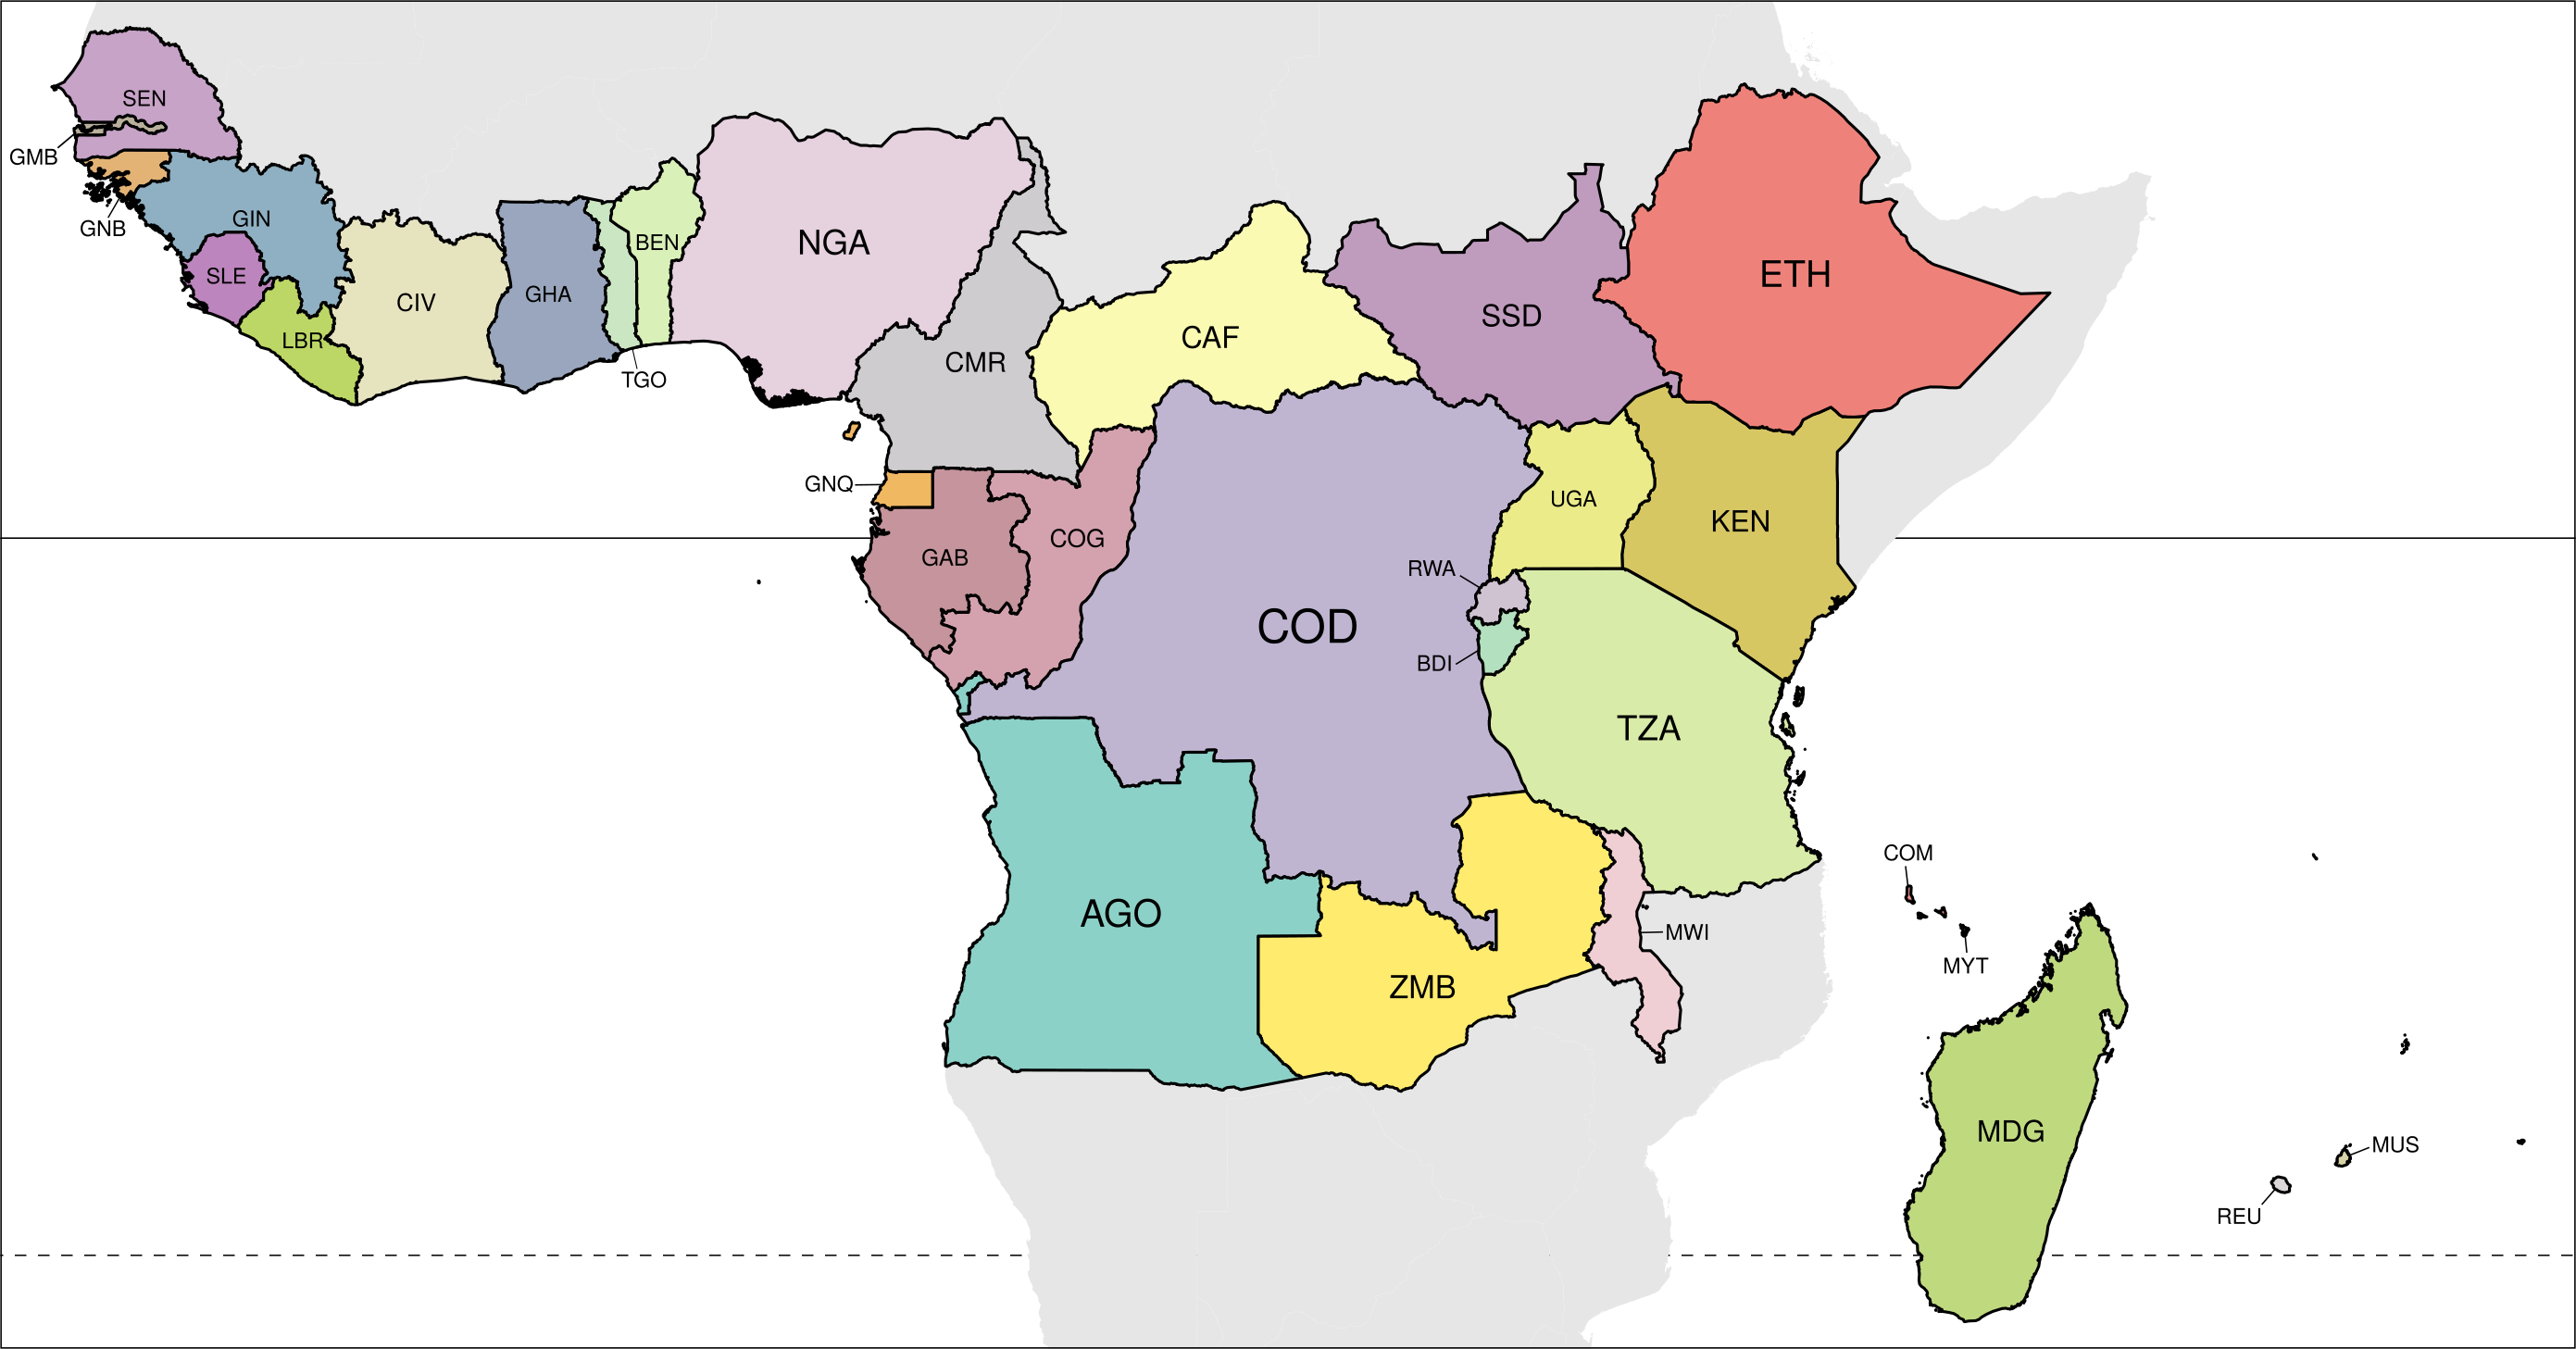
\includegraphics[width=0.32\textwidth]{figs/sm/study_areas_Africa}
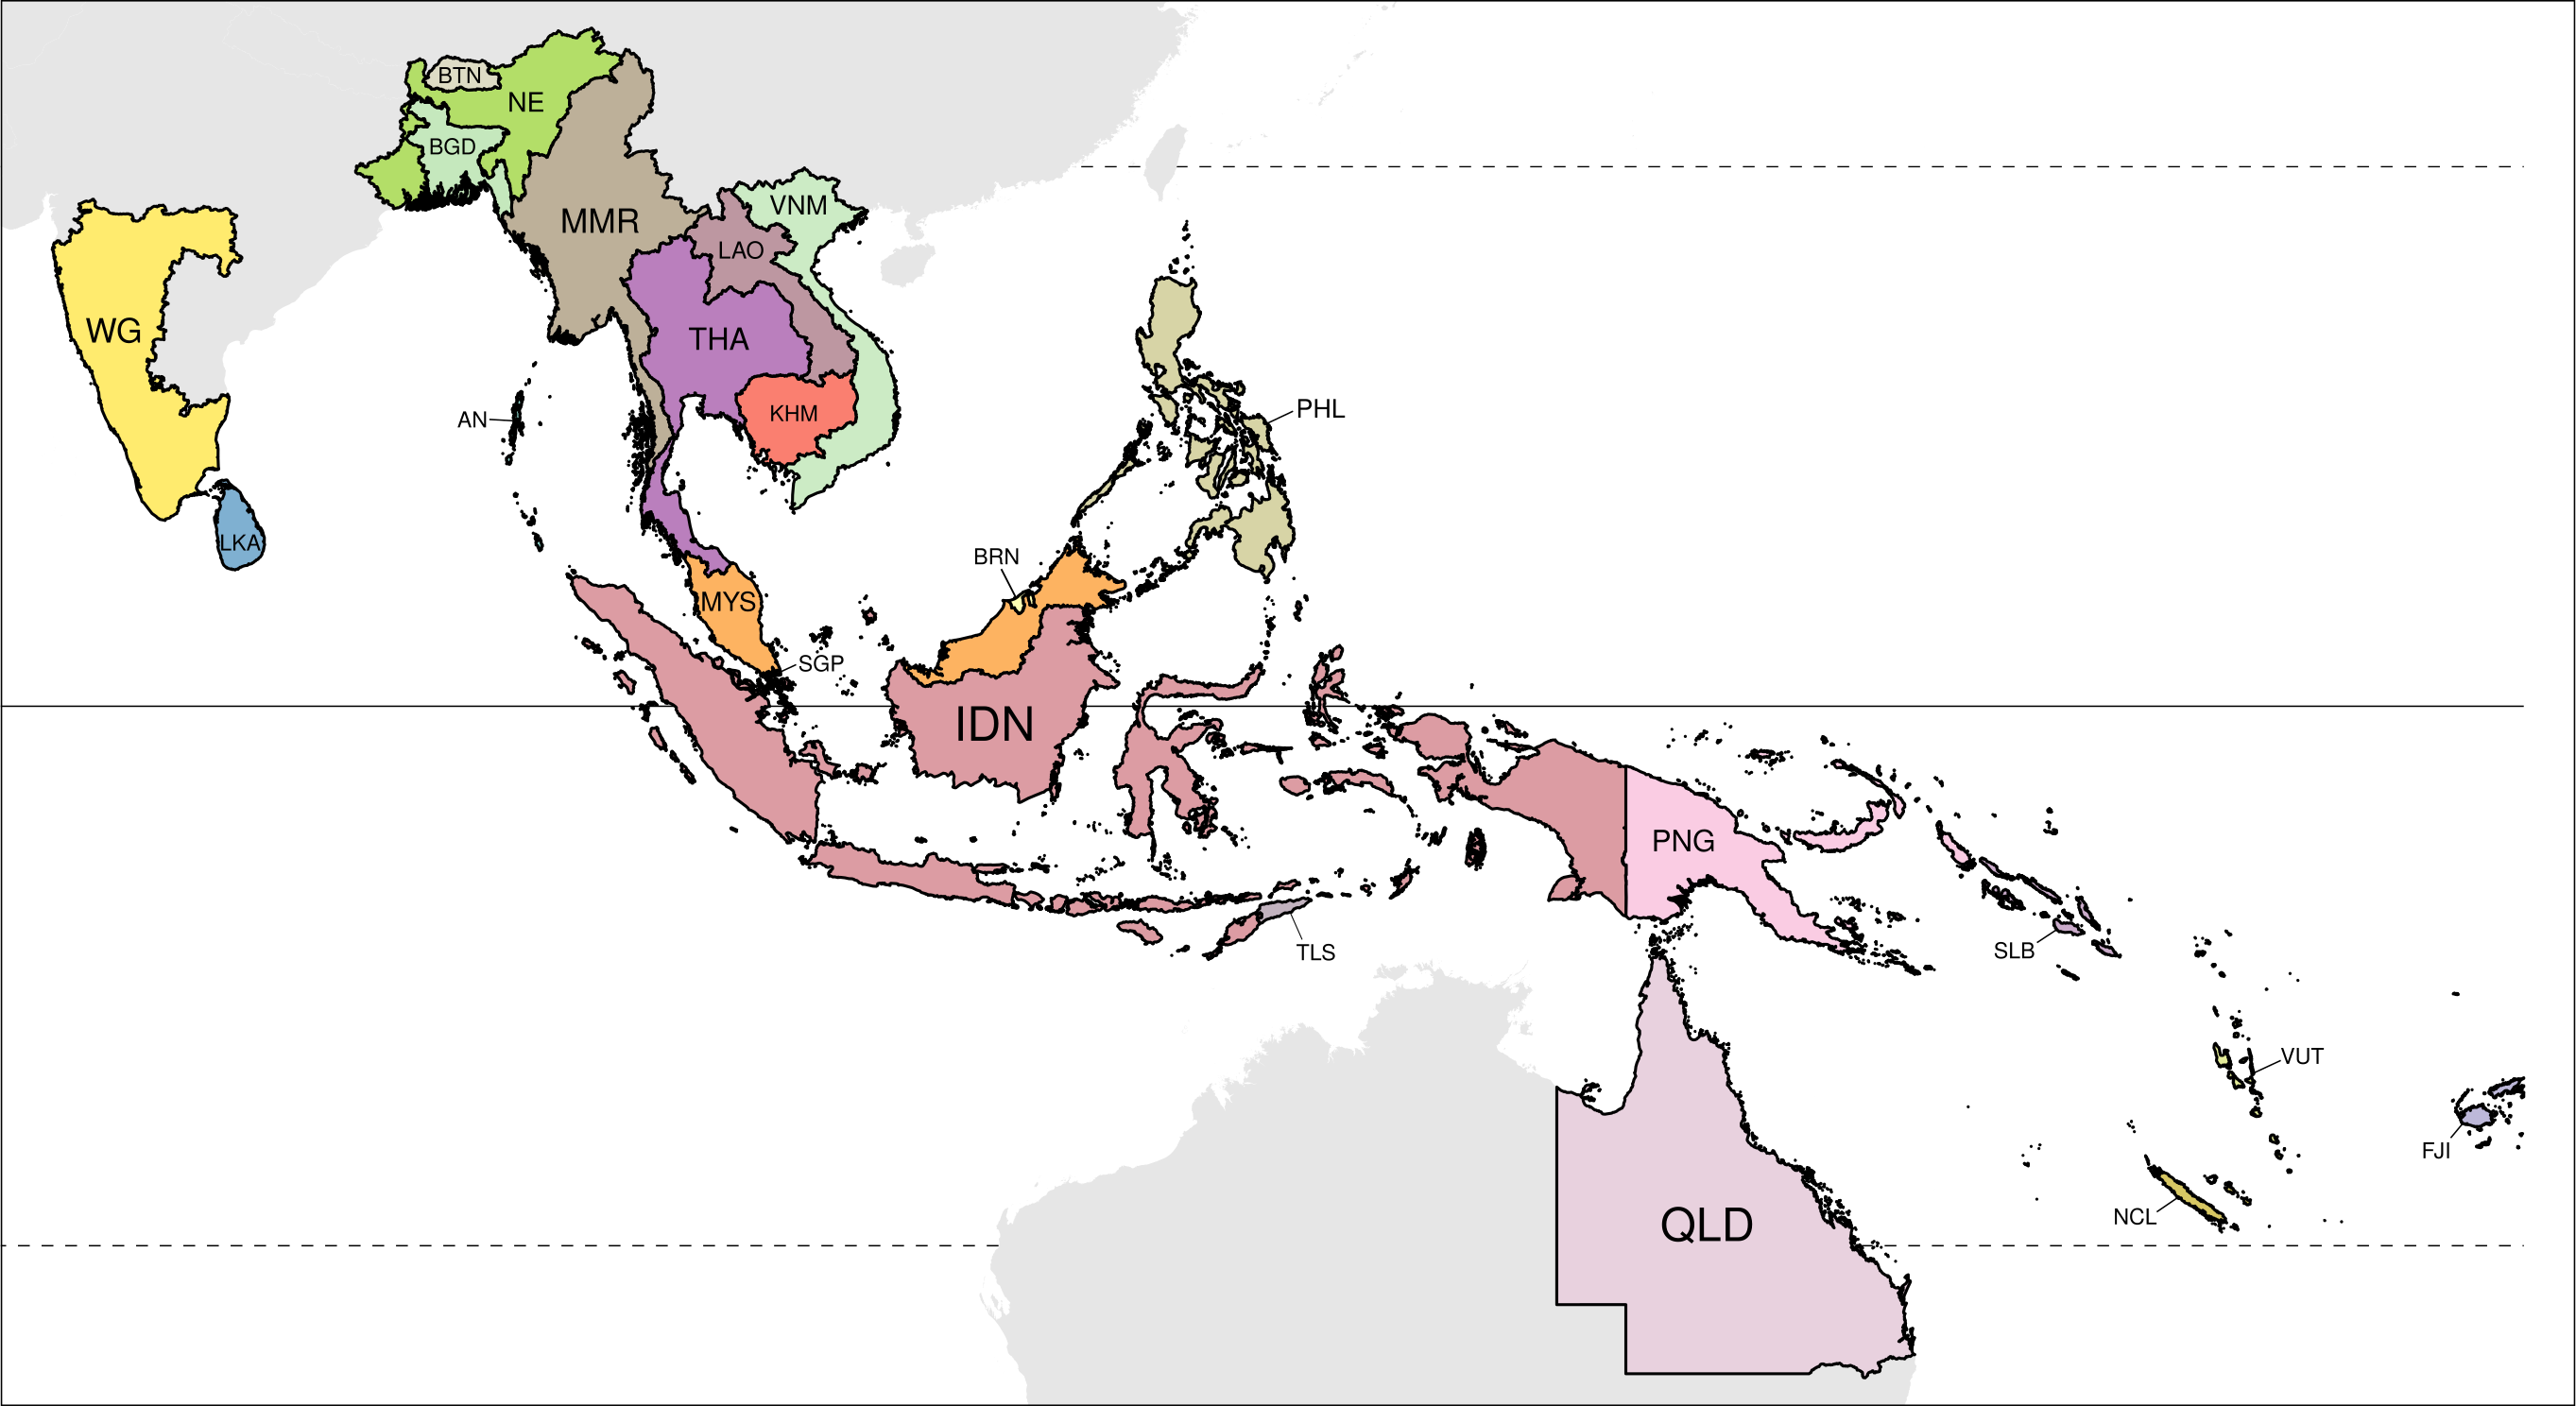
\includegraphics[width=0.32\textwidth]{figs/sm/study_areas_Asia}
\textbf{Les 119 zones d'étude sur les 3 continents}
\end{center}
\end{frame}

\begin{frame}[label={sec:org0624b06}]{ForestAtRisk in the tropics}
\begin{center}
\includegraphics[width=0.7\textwidth]{figs/article/prob.png}
\end{center}

\textbf{Carte pantropicale de la probabilité spatiale de déforestation}

Article en cours de révision :
\href{https://doi.org/10.1101/2022.03.22.485306}{10.1101/2022.03.22.485306}

\url{https://forestatrisk.cirad.fr/maps.html}
\end{frame}

\subsection{Modèles à fenêtre mobile}
\label{sec:orgbbb3a86}

\begin{frame}[label={sec:orgd351244}]{Modèles à fenêtre mobile}
\begin{itemize}
\item Modèle proposé par la méthodologie précédente de Verra.
\item Trouver un seuil de distance pour définir la classe 1 pour le risque de
déforestation (même chose que pour le modèle de référence).
\end{itemize}

\begin{columns}
\begin{column}{0.55\NLargeur de colonne}
\begin{figure}[htbp]
\centering
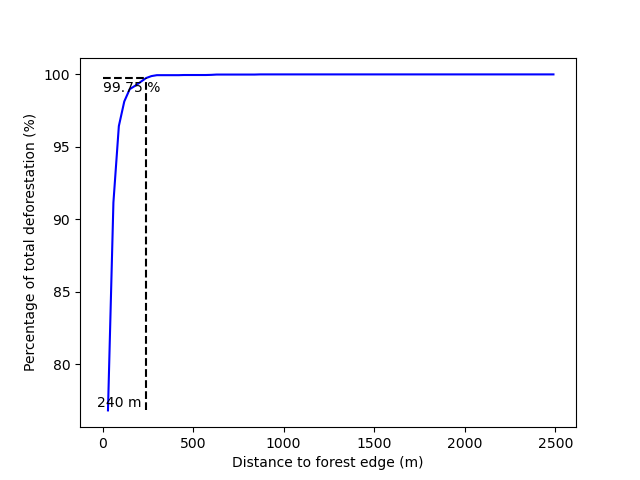
\includegraphics[width=\textwidth]{figs/get_started/perc_dist.png}
\caption{Déforestation cumulée en fonction de la distance à la lisière de la forêt.}
\end{figure}
\end{column}

\begin{column}{0.45\NLargeur de colonne}
\begin{center}
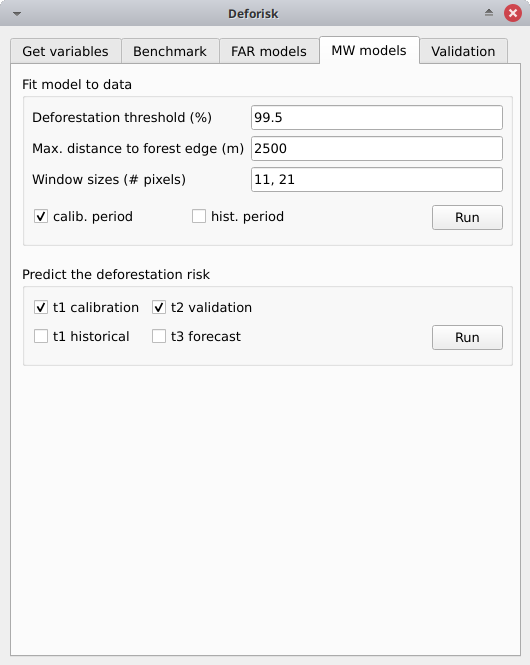
\includegraphics[width=0.9\textwidth]{figs/plugin_api/interface_mw_models.png}
\end{center}
\end{column}
\end{columns}
\end{frame}

\begin{frame}[label={sec:org97be5e1}]{Modèles à fenêtre mobile}
\begin{itemize}
\item Calculer un risque local de déforestation au niveau du pixel à l'aide d'une
fenêtre mobile.
\item La fenêtre mobile peut être de différentes tailles.
\item Les taux de déforestation dans [0, 1] sont convertis en [2, 65535].
\end{itemize}

\begin{figure}[htbp]
\centering
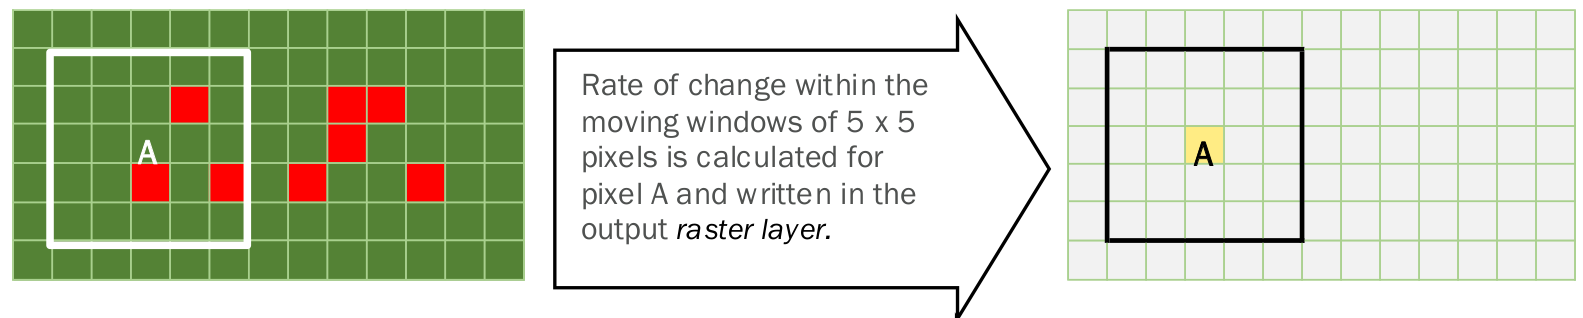
\includegraphics[width=0.8\textwidth]{figs/moving_window.png}
\caption{Fenêtre mobile.}
\end{figure}
\end{frame}

\subsection{Validation}
\label{sec:org384bc69}

\begin{frame}[label={sec:org2b0ec9c}]{Validation}
\begin{columns}
\begin{column}{0.5\columnwidth}
\begin{itemize}
\item Comparaison entre la déforestation prévue et la déforestation observée (en
ha) pour chaque cellule d'une grille grossière.
\item Pour une période donnée.
\end{itemize}
\begin{center}
\includegraphics[width=0.7\textwidth]{figs/grid.png}
\end{center}  
\end{column}
\begin{column}{0.5\columnwidth}
\begin{center}
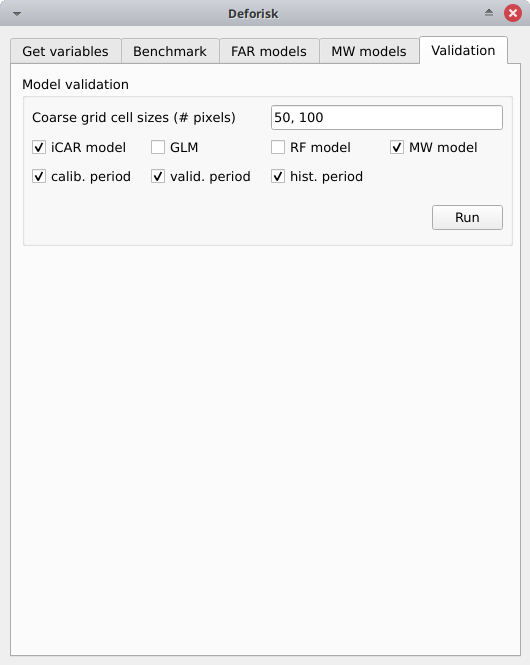
\includegraphics[width=\textwidth]{figs/plugin_api/interface_validation.png}
\end{center}
\end{column}
\end{columns}
\end{frame}

\begin{frame}[label={sec:org3609995}]{Validation}
\begin{itemize}
\item Indices de performance : \(R^2\), et médiane de l'erreur absolue (MedAE).
\item Calculé pour chaque modèle et chaque période (calibration, validation,
historique).
\end{itemize}

\begin{center}
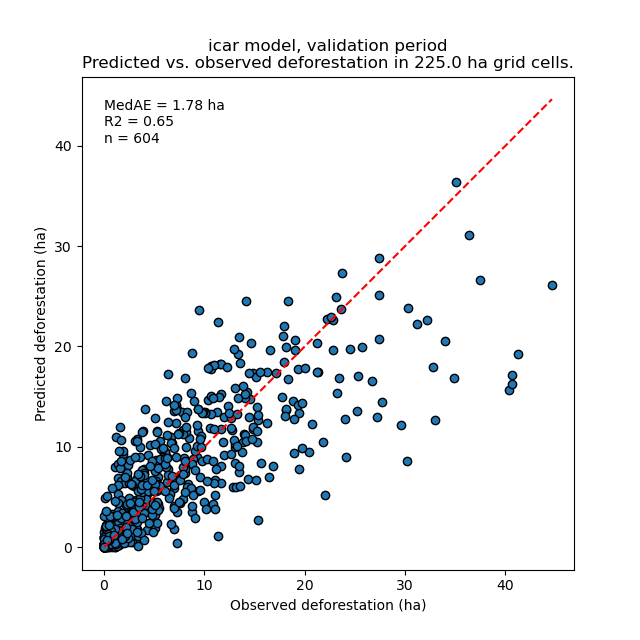
\includegraphics[width=0.6\textwidth]{figs/get_started/pred_obs_icar_validation_50.png}
\end{center}
\end{frame}

\section{Utilisation}
\label{sec:org3edfc8e}

\subsection{Attribution de la déforestation}
\label{sec:org9fb3dab}

\begin{frame}[label={sec:orgff8474c}]{Attribution de la déforestation}
For the best model, we obtain at t3:
\begin{itemize}
\item Une carte juridictionnelle avec des classes de risque de déforestation.
\item Un tableau des taux de déforestation relatifs pour chaque classe.
\end{itemize}

\begin{table}[htbp]
\caption{\label{tab-defrate}Taux de déforestation à t3 pour chaque classe de risque de déforestation
(nombres tronqués à trois chiffres après la virgule).}
\petit
\begin{tabular}{rrlrllrl}
\toprule cat & \(n_i\) & \(d_i\) & \(\theta_{m,i}\) & \(\theta_{a,i}\) & \(T\) & \(A\) & \(\delta_{i}\)\\[0pt] \N- La règle du milieu 1 & 137575 & -- & 1.000e-06 & -- & -- & 0.09 & --\\[0pt] 2 & 5425 & -- & 1.625e-05 & -- & -- & 0.09 & --\\[0pt] 3 & 3523 & -- & 3.151e-05 & -- & -- & 0.09 & --\\[0pt] 4 & 2458 & -- & 4.677e-05 & -- & -- & 0.09 & --\\[0pt] 5 & 2078 & -- & 6.203 & -- & -- & 0.09 & --\\[0pt] \N- La règle du bas
\end{tabular}
\end{table}
\end{frame}

\begin{frame}[label={sec:org6aa68e5}]{Attribution de la déforestation}
\begin{table}[htbp]
\caption{\label{tab-defrate-header}Taux de déforestation à t3 pour chaque classe de risque de déforestation
(nombres tronqués à trois chiffres après la virgule).}
\petit
\begin{tabular}{rrlrllrl}
\toprule cat & \(n_i\) & \(d_i\) & \(\theta_{m,i}\) & \(\theta_{a,i}\) & \(T\) & \(A\) & \(\delta_{i}\)\\[0pt] \N- La règle du milieu 1 & 137575 & -- & 1.000e-06 & -- & -- & 0.09 & --\\[0pt] \N- La règle du bas
\end{tabular}
\end{table}

\begin{itemize}
\item Envisager un total de{deforestation} (en hectares) pour les prochaines
années (en années){years} au niveau juridictionnel.
\item \textbf{facteur d'ajustement} est \rho = D / (A \sum_i n_{i}
\theta_{m,i})\), avec \(A\) la surface du pixel en ha.
\item \textbf{Taux absolu} est \(\theta_{a,i} = \rho \theta_{m,i}\) : de sorte que
la déforestation totale prédite = la déforestation attendue.
\item \textbf{Densité de déforestation} est \(\delta_{i} = \theta_{a,i} \times A /
Y\). Utilisé pour prédire la quantité de déforestation (en ha/an) pour
chaque pixel de forêt.
\end{itemize}
\end{frame}

\begin{frame}[label={sec:orge68269d}]{Attribution de la déforestation}
\textbf{Deforestation density} is \(\delta_{i}\) (in ha/yr) is used to
predict the amount of deforestation for each forest pixel.

\begin{figure}[htbp]
\centering
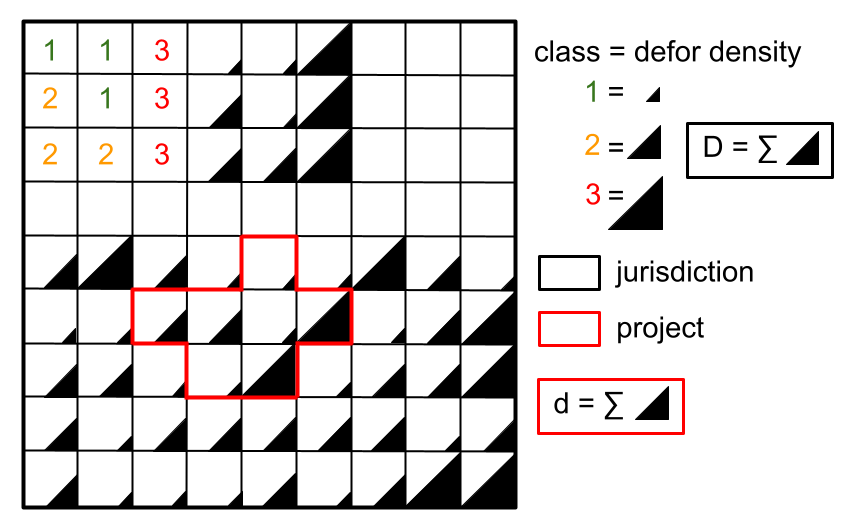
\includegraphics[width=8cm]{figs/get_started/allocation.png}
\caption{Affectation de la déforestation à des projets relevant de la juridiction.}
\end{figure}
\end{frame}

\subsection{Juridictions infranationales}
\label{sec:orgada2c1e}

\begin{frame}[label={sec:org6424960},fragile]{Juridictions infranationales}
 \begin{itemize}
\item Possibilité de travailler avec des juridictions infranationales.
\item Fichier GPKG nommé \texttt{aoi\_latlon.gpkg} avec deux couches nommées
\texttt{aoi} pour la juridiction et \texttt{subj} pour les sous
juridictions.
\item Ce fichier peut ensuite être utilisé avec le plugin \texttt{deforisk} pour
définir la zone d'intérêt (AOI).
\item Plus de détails sur la page du site web
\href{https://deforisk-qgis-plugin.org/articles/subnational\_jurisd.html}{Subnational
jurisdictions}.
\end{itemize}

\begin{center}
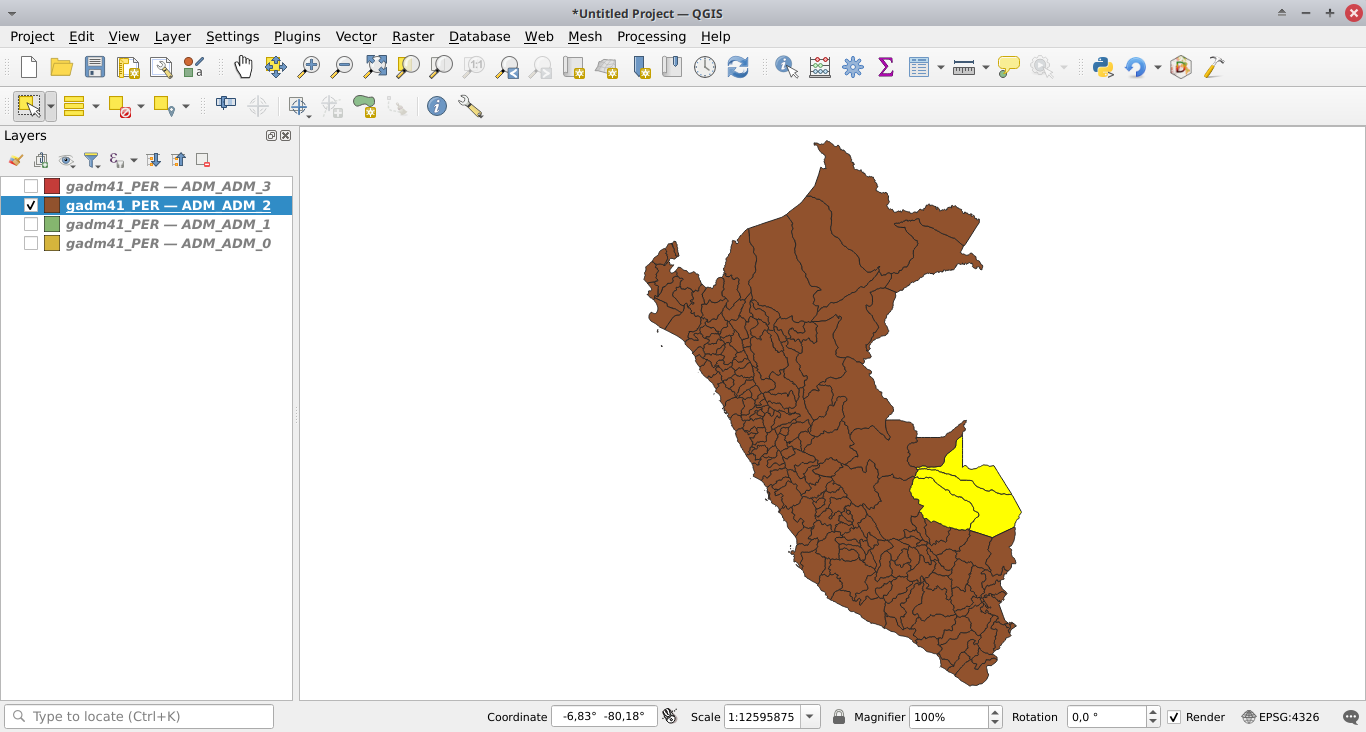
\includegraphics[width=7cm]{figs/select_subjurisdictions.png}
\end{center}
\end{frame}

\subsection{Données de l'utilisateur}
\label{sec:org6992bcf}

\begin{frame}[label={sec:orgd079d9f},fragile]{Données de l'utilisateur}
 \begin{itemize}
\item Possibilité d'utiliser les données de l'utilisateur : carte des changements
du couvert forestier national, autres variables explicatives (par exemple,
concessions minières).
\item Pour l'instant, il s'agit d'étapes manuelles.
\item Les fichiers du dossier \texttt{data} doivent être remplacés par les données
de l'utilisateur.
\item Des variables matricielles supplémentaires peuvent être ajoutées au dossier
\texttt{data}.
\item Les liens symboliques dans les dossiers \texttt{data\_*} doivent exister.
\item Plus de détails sur la page du site web
\href{https://deforisk-qgis-plugin.org/articles/user\_data.html}{Données
utilisateur}.
\end{itemize}
\end{frame}

\section{Conclusion}
\label{sec:org8b1578c}

\subsection{Ordre du jour de l'atelier}
\label{sec:org9e257b5}

\begin{frame}[label={sec:orgc45bd60},fragile]{Ordre du jour de l'atelier}
 Four practical sessions:

\begin{itemize}
\item Installer le logiciel et exécuter le tutoriel \texttt{Get Started}.
\item Choisissez une petite juridiction infranationale et sélectionnez la
meilleure carte des risques.
\item Déterminer la meilleure carte des risques pour une grande juridiction (par
exemple, à l'échelle d'un pays).
\item Exercices :
\begin{itemize}
\item Modifier les paramètres du modèle pour voir le comportement des modèles (par
exemple, la taille des cellules spatiales pour le modèle iCAR).
\item Utiliser des données nationales (par exemple, la carte nationale des
changements du couvert forestier).
\item Attribuer la déforestation future à un projet.
\end{itemize}
\end{itemize}
\end{frame}

\subsection{Perspectives}
\label{sec:org679384f}

\begin{frame}[label={sec:org1c4e543}]{Perspectives}
\begin{itemize}
\item Plugin récent (première version en juillet 2024).
\item Des améliorations sont attendues :
\begin{itemize}
\item Augmenter la vitesse de calcul (pour les prédictions sur de grandes zones).
\item Ajout de modèles alternatifs (MLP).
\end{itemize}
\item Modifications en fonction du retour d'information des utilisateurs.
\end{itemize}
\end{frame}


{ \Nmodèle d'arrière-plan{\Nincludegraphics[keepaspectratio=true,
height=\paperheight]{figs/Canopy-NC}} } \setbeamertemplate{symboles de
navigation}{} \setbeamertemplate{blocks}[rounded][shadow=false]
\begin{frame}[plain] \vspace*{\stretch{100}} \begin{block}{} \begin{center}
\ldots~Merci de votre attention~\ldots \\N- \N- \N- \N- \N- \N- \N- \N-
\N-{COPY00} \\N-textbf{> Articles > Références > Présentations} \\ 

\includegraphics[width=0.8\textwidth]{figs/partners_logos} \end{center}
\end{block} \end{frame} }
\end{document}
